\documentclass[12pt]{article}
\usepackage{amsmath}
\usepackage{amsthm}
\usepackage{amssymb}
\usepackage{euscript}
\usepackage{mathrsfs}
\usepackage{bm}
\usepackage{enumitem}
\usepackage{tikz}
\usepackage{mathtools}
\usepackage{float}
\usepackage{hyperref}
\usepackage{boldline}
\usepackage{indentfirst}
\usepackage{environ}
\usepackage{courier}
\usetikzlibrary{positioning}

\renewcommand{\labelitemii}{$\vartriangleright$}
\renewcommand{\labelitemiv}{$\Join$}

\makeatletter
\newsavebox{\measure@tikzpicture}
\NewEnviron{scaletikzpicturetowidth}[1]{%
  \def\tikz@width{#1}%
  \def\tikzscale{1}\begin{lrbox}{\measure@tikzpicture}%
  \BODY
  \end{lrbox}%
  \pgfmathparse{#1/\wd\measure@tikzpicture}%
  \edef\tikzscale{\pgfmathresult}%
  \BODY
}
\makeatother

\numberwithin{equation}{section}

\hypersetup{
    colorlinks=true,
    % linkcolor=blue,
    linkcolor=[RGB]{0,0,128},
    % filecolor=[RGB]{0,0,128},
    filecolor=magenta,
    urlcolor=cyan,
    citecolor = [RGB]{128,0,128}
}

\newcommand{\myref}[2]{\hyperref[#2]{#1 \ref*{#2}}}
\newcommand{\myrefT}[1]{\hyperref[#1]{Theorem \ref*{#1}}}
\newcommand{\myrefP}[1]{\hyperref[#1]{Proposition \ref*{#1}}}
\newcommand{\myrefL}[1]{\hyperref[#1]{Lemma \ref*{#1}}}
\newcommand{\myrefD}[1]{\hyperref[#1]{Definition \ref*{#1}}}
\newcommand{\myrefn}[3]{\hyperref[#2]{#1 \ref*{#2} (#3)}}

% \input{dynkinMacros.tex}
% \input{dynkinEMacros.tex}
% \renewcommand{\qedsymbol}{}
\newcommand{\ssm}{\smallsetminus}

\newcommand{\para}[1]{\noindent\underline{#1}.}

\newcommand{\ti}{$\tau\textnormal{-invariant}$}
\newcommand{\prim}{\textnormal{Prim}_{\lambda}(\textnormal{U}(\gf))}

\newcommand{\ve}{\varepsilon}
\newcommand{\veo}{\varepsilon_1}
\newcommand{\vet}{\varepsilon_2}
\newcommand{\vei}{\varepsilon_i}
\newcommand{\vp}{\varphi}

% \newcommand{\inr}{\textnormal{In}^R}
% \newcommand{\inl}{\textnormal{In}^L}
% \newcommand{\inc}{\textnormal{In}}
% \renewcommand{\sc}{\textnormal{SC}}
% \newcommand{\re}{\textnormal{Re}}

\newcommand{\ag}{\alpha}
\newcommand{\bg}{\beta}
\newcommand{\g}{\gamma}
\newcommand{\dg}{\delta}
\newcommand{\rg}{\rho}
\newcommand{\kg}{\kappa}
\newcommand{\sg}{\sigma}
\newcommand{\tg}{\tau}
\renewcommand{\lg}{\lambda}

\renewcommand{\gg}{$\gamma \ $}
\newcommand{\ga}{$\alpha \ $}
\newcommand{\gt}{$\tau $}
\renewcommand{\(}{(\gamma)}
\newcommand{\atg}{\tilde\alpha}
\newcommand{\ags}[1]{{\ag_{#1}}}
\newcommand{\ao}{{\ag_1'}}

\newcommand{\gf}{\mathfrak g}
\newcommand{\hf}{\mathfrak h}

% needs a new name
%\newcommand{\th}[1]{{$\text{\it #1 }^{\underline{\textnormal{th}}}$}}
\renewcommand{\sf}{\mathscr F}
\newcommand{\dsf}{$\sf$}
\newcommand{\st}{\mathscr T}
% needs a new name  -- ok?
\newcommand{\so}[1]{\mathscr #1}


\newcommand{\snn}{{\mathscr S(n,n)}}
\newcommand{\smm}{{\mathscr S(M^L,M^R)}}
\renewcommand{\tan}{\mathscr T_A(n)}
\newcommand{\tn}{\mathscr T(n)}
\newcommand{\dtn}{$\tn$}
\newcommand{\tm}{\mathscr T(M)}
\newcommand{\dtm}{$\tm$}
\newcommand{\tcsn}{\mathscr T_C^S(n)}
\newcommand{\tbsn}{\mathscr T_B^S(n)}
\newcommand{\tsn}[1]{\mathscr T_#1(n)}
\newcommand{\tsm}[1]{\mathscr T_#1(M)}
\newcommand{\tnn}{\mathscr T(n,n)}
\newcommand{\tmm}{\mathscr T(M^L,M^R)}
\newcommand{\tkmm}{\mathscr T_K(M^L,M^R)}
\newcommand{\tsnn}[1]{\mathscr T_#1(n,n)}
\newcommand{\tsmm}[1]{\mathscr T_#1(M^L,M^R)}
\newcommand{\tdnn}{\mathscr T_D(n,n)}
\newcommand{\tdmm}{\mathscr T_D(M^L,M^R)}
\newcommand{\tdn}{\mathscr T_D(n)}
\newcommand{\tdm}{\mathscr T_D(M)}
\newcommand{\tcnn}{\mathscr T_C(n,n)}
\newcommand{\tcmm}{\mathscr T_C(M^L,M^R)}
\newcommand{\tcn}{\mathscr T_C(n)}
\newcommand{\tcm}{\mathscr T_C(M)}
\newcommand{\cm}{\mathscr C(M)}
\newcommand{\dm}{\mathscr D(M)}

\newcommand{\snnp}{\mathscr S'(n,n)}
\newcommand{\smmp}{\mathscr S'(M^L,M^R)}
\newcommand{\snnpp}{\mathscr S''(n,n)}
\newcommand{\smmpp}{\mathscr S''(M^L,M^R)}
\newcommand{\tnnp}{\mathscr T'(n,n)}
\newcommand{\tmmp}{\mathscr T'(M^L,M^R)}
\newcommand{\tnnpp}{\mathscr T''(n,n)}
\newcommand{\tmmpp}{\mathscr T''(M^L,M^R)}
\newcommand{\tdnnp}{\mathscr T_D'(n,n)}
\newcommand{\tdmmp}{\mathscr T_D'(M^L,M^R)}
\newcommand{\tdnnpp}{\mathscr T_D''(n,n)}
\newcommand{\tdmmpp}{\mathscr T_D''(M^L,M^R)}


\newcommand{\talb}{T_{\alpha \beta}}
\newcommand{\tai}{T_{\alpha_i,\alpha_{i+1}}}
\newcommand{\tap}{T_{\alpha_{i+1},\alpha_i}}
\newcommand{\tao}{T_{\alpha_1,\alpha_2}}
\newcommand{\tat}{T_{\alpha_2,\alpha_1}}

% new
\newcommand{\talbLeft}{T^L_{\alpha \beta}}
\newcommand{\talbRight}{T^R_{\alpha \beta}}

\newcommand{\ot}{\overline T}
\newcommand{\og}{\overline{\gamma}}

\newcommand{\sij}{{S_{ij}}}
\renewcommand{\ss}[2]{{S_{#1,#2}}}
% \def\ss#1#2{S_{#1,#2}}

\newcommand{\im}{{i-1}}
% \renewcommand{\ip}{{i+1}}
\newcommand{\ip}{{i+1}}
\newcommand{\imm}{{i-2}}
\newcommand{\ipp}{{i+2}}
\newcommand{\jm}{{j-1}}
\newcommand{\jp}{{j+1}}
\newcommand{\jmm}{{j-2}}
\newcommand{\jpp}{{j+2}}

\renewcommand{\tt}{\tau (T)}
\newcommand{\abe}{{$\{\ag,\bg\}=\{\ag_i,\ag_\ip\}$}}

\newcommand{\bt}{\mathbf T}
\newcommand{\bto}{\mathbf T_1}
\newcommand{\btt}{\mathbf T_2}
\newcommand{\obt}{\overline\bt}
\newcommand{\obto}{\overline\bt_1}
\newcommand{\obtt}{\overline\bt_2}
\newcommand{\tbt}{\tilde\bt}
\newcommand{\tbto}{\tilde\bto}
\newcommand{\tbtt}{\tilde\btt}
\newcommand{\pbt}{(\bto,\btt)}
\newcommand{\pbtp}{(\bto',\btt')}
\newcommand{\pobt}{(\obto,\obtt)}
\newcommand{\pbts}[1]{(\bto^{#1},\btt^{#1})}
\newcommand{\pobts}[1]{(\obto^{#1},\obtt^{#1})}
\newcommand{\pobtp}{(\obto',\obtt')}

\newcommand{\lo}{(\bto,\bt)}
\newcommand{\lop}{(\bto',\bt)}
\newcommand{\ls}[1]{(\bt_#1,\bt)}
\newcommand{\lsp}[1]{(\bt_#1',\bt)}
\newcommand{\ol}{(\obt_1,\obt)}

\newcommand{\be}{\mathbf E}
\newcommand{\bs}{\mathbf S}
\newcommand{\bl}{\mathbf L}
\newcommand{\br}{\mathbf R}
% \renewcommand{\op}{\bar P}
\newcommand{\op}{\bar P}
\newcommand{\pe}{P_e}

\newcommand{\oc}{\overline c}
\newcommand{\cL}{\prescript{L}{}{c}}
\newcommand{\cR}{\prescript{R}{}{c}}
\newcommand{\bc}{\mathbf c}
\newcommand{\bcL}{\prescript{L}{}{\bc}}
\newcommand{\bcR}{\prescript{R}{}{\bc}}
\newcommand{\overbc}{\overline{\mathbf c}}
\newcommand{\overcL}{\prescript{L}{}{\overline c}}
\newcommand{\overcR}{\prescript{R}{}{\overline c}}
\newcommand{\overbcL}{\prescript{L}{}{\overbc}}
\newcommand{\overbcR}{\prescript{R}{}{\overbc}}

% \newcommand{\sha}{{\textnormal{Shape}}}
\newcommand{\cs}{{c.s.p.b.}}
% \newcommand{\OC}{{\textnormal{OC}}}
% \newcommand{\OCS}{{\textnormal{OC*}}}
\newcommand{\Sf}{S_f}
\newcommand{\Sb}{S_b}
\newcommand{\nh}{n_h}
\newcommand{\nv}{n_v}
\newcommand{\rinf}{\rg_{\inf}}
\newcommand{\rsup}{\rg_{\sup}}

\newcommand{\ec}{\underset {ec}\sim}
\newcommand{\gtl}{\underset {GTL}\sim}
\newcommand{\en}{\underset {n}\sim}
\newcommand{\enm}{\underset {n-1}\sim}
\newcommand{\eqm}{\underset {m}\sim}
\newcommand{\eqmm}{\underset {m-1}\sim}
\newcommand{\ez}{\underset {0}\sim}
\newcommand{\gtr}{\underset {GTR}\sim}
\renewcommand{\gt}{\underset {GT}\sim}
\newcommand{\ngtl}{\underset {GTL}\nsim}
\newcommand{\jl}{\underset {JL}\sim}
\newcommand{\jr}{\underset {JR}\sim}
\newcommand{\kll}{\underset {KLL}\sim}
\newcommand{\klr}{\underset {KLR}\sim}

\newcommand{\fo}{F_1}
\newcommand{\ft}{F_2}
\newcommand{\fot}{\tilde\fo}
\newcommand{\ftt}{\tilde\ft}

\newcommand{\bi}{{\it b}){\it i})}
\newcommand{\bii}{{\it b}){\it ii})}

\newcommand{\sig}{\Sigma}
\newcommand{\tsl}{T_\Sigma^L}
\newcommand{\tspl}{T_{\Sigma'}^L}
\newcommand{\tssl}[1]{T_{\Sigma^#1}^L}
\newcommand{\tssbl}[1]{T_{\Sigma_#1}^L}
\newcommand{\ts}{T_\Sigma}
\newcommand{\tsp}{T_{\Sigma'}}
\newcommand{\tss}[1]{T_{\Sigma^#1}}
\newcommand{\tssb}[1]{T_{\Sigma_#1}}
\newcommand{\pin}{$\Pi\ssm\{\ag_n\}$}
\newcommand{\pc}{\phi_C}
% \newcommand{\pd}{{\phi_D}}
\newcommand{\il}{I_\lg}

\newcommand{\te}[1]{\textnormal{#1}}

\newcommand{\plainTL}{\prescript{L}{}{T}}
\newcommand{\plainTR}{\prescript{R}{}{T}}

\newcommand{\tL}{\prescript{L}{}{\bt}}
\newcommand{\tR}{\prescript{R}{}{\bt}}
\newcommand{\pairTLR}{(\tL,\tR)}
\newcommand{\pairTLRPrime}{(\tL',\tR')}
\newcommand{\pairTLRSub}[1]{(\tL_{#1},\tR_{#1})}
\newcommand{\pairTLRPrimeSub}[1]{(\tL'_{#1},\tR'_{#1})}

\newcommand{\overTL}{\prescript{L}{}{\obt}}
\newcommand{\overTR}{\prescript{R}{}{\obt}}
\newcommand{\overPairTLR}{(\overTL,\overTR)}
\newcommand{\overPairTLRPrime}{(\overTL',\overTR')}
\newcommand{\overPairTLRSub}[1]{(\overTL_{#1},\overTR_{#1})}
\newcommand{\overPairTLRPrimeSub}[1]{(\overTL'_{#1},\overTR'_{#1})}

\newcommand{\tildeTL}{\prescript{L}{}{\tbt}}
\newcommand{\tildeTR}{\prescript{R}{}{\tbt}}
\newcommand{\tildePairTLR}{(\tildeTL, \tildeTR)}
\newcommand{\pairTLRStar}{(\tL^*, \tR^*)}
\newcommand{\overPairTLRStar}{(\overTL^*, \overTR^*)}

\newcommand{\pisn}{{$\Pi^*\ssm\{\ag_n\}$}}

\newcommand{\tLSigma}{\tsl}
\newcommand{\tLSigmaSub}[1]{\tssbl#1}
\newcommand{\tDMM}{\tdmm}

\newcommand{\leftPrime}{(\tL',\tR)}
\newcommand{\leftSub}[1]{(\tL_{#1},\tR)}
\newcommand{\leftPrimeSub}[1]{(\tL_{#1}',\tR)}


\DeclareMathOperator{\Shape}{Shape}
\DeclareMathOperator{\OC}{OC}
\DeclareMathOperator{\OCS}{OC*}
% \newcommand{\inr}{\textnormal{In}^R}
% \newcommand{\inl}{\textnormal{In}^L}
% \newcommand{\inc}{\textnormal{In}}
% \renewcommand{\sc}{\textnormal{SC}}
\newcommand{\re}{\textnormal{Re}}
\DeclareMathOperator{\In}{In}
\newcommand{\inc}{\In}
\newcommand{\inL}{\In^L}
\newcommand{\inR}{\In^R}
\DeclareMathOperator{\SC}{SC}
\newcommand{\scL}{\SC^L}
\newcommand{\scR}{\SC^R}

\DeclareMathOperator{\Adj}{Adj}
\newcommand{\oeta}{\overline{\eta}}

\newcommand{\preL}[1]{\prescript{L}{}{#1}}

\newcommand{\makeBox}[2] {
  \newsavebox{#1}
  \begin{lrbox}{#1}{#2}\end{lrbox}
}

\tikzstyle{tableau} = [y = -1cm, every node/.style={transform shape}]

\definecolor{gridColor}{RGB}{19,83,150}
\tikzstyle{dominoStyle} = [color=black, fill=white, rounded corners = .1cm, thick]
\tikzstyle{gridLine} = [color=gridColor, thick]
\tikzstyle{dominoText} = [font=\Large, midway]
\tikzstyle{cycleLine} = [color=green, thick, >->]
\tikzstyle{closedCycleLine} = [color=green, thick]
% \tikzstyle{fixedSquareStyle} = [pattern = crosshatch doats, pattern color=gridColor,  opacity=0.2]
\tikzstyle{fixedSquareStyle} = [color=gridColor,  opacity=0.07]
\tikzstyle{tileText} = [font=\large, midway]

\newcommand{\eps}{.06}
\newcommand{\teps}{\eps * 2}

% first entry is row, starting with 1, second entry is column, third is content
\newcommand{\filledSquare}[3]{\filldraw [dominoStyle] (#2 - 1 + \eps, #1 - 1 + \eps) rectangle + (1 - \teps, 1 -\teps) node [tileText] {$#3$};}
% The fourth entry shifts vertically
\newcommand{\filledSquareShift}[4]{\filldraw [dominoStyle] (#2 - 1 + #4 + \eps, #1 - 1 + \eps) rectangle + (1 - \teps, 1 -\teps) node [tileText] {$#3$};}

\newcommand{\horizontalDomino}[3]{\filldraw [dominoStyle] (#2 - 1 + \eps, #1 - 1 + \eps) rectangle + (2 - \teps, 1 -\teps) node [dominoText] {$#3$};}
\newcommand{\verticalDomino}[3]{\filldraw [dominoStyle] (#2 - 1 + \eps,  #1 - 1 + \eps) rectangle + (1 - \teps,2 -\teps) node [dominoText] {$#3$};}

\newcommand{\horizontalDominoShift}[4]{\filldraw [dominoStyle] (#2 - 1 + #4 + \eps, #1 - 1 + \eps) rectangle + (2 - \teps, 1 -\teps) node [dominoText] {$#3$};}
\newcommand{\verticalDominoShift}[4]{\filldraw [dominoStyle] (#2 - 1 + #4 + \eps,  #1 - 1 + \eps) rectangle + (1 - \teps,2 -\teps) node [dominoText] {$#3$};}

\newcommand{\zeroSquare}[2]{\filldraw [dominoStyle] (#2 - 1 + \eps, #1 - 1 + \eps) rectangle + (1 - \teps, 1 -\teps) node [dominoText] {$0$};}
\newcommand{\zeroSquareShift}[3]{\filldraw [dominoStyle] (#2 - 1 + #3 + \eps, #1 - 1 + \eps) rectangle + (1 - \teps, 1 -\teps) node [dominoText] {$0$};}


\newcommand{\emptyBox}[2]{\filldraw [dominoStyle] (#2 - 1 + \eps, #1 - 1 + \eps) rectangle + (2 - \teps, 2 -\teps);}
\newcommand{\signedBox}[3]{
\filldraw [opacity=0] (#2 - 1 + 1, #1 - 1) rectangle + (1, 2) node [dominoText,opacity=1] {$#3$};
\filldraw [dominoStyle, fill opacity = 0] (#2 - 1 + \eps, #1 - 1 + \eps) rectangle + (2 - \teps, 2 -\teps);
}

\newcommand{\emptyBoxShift}[3]{\filldraw [dominoStyle] (#2 - 1 + #3 + \eps, #1 - 1 + \eps) rectangle + (2 - \teps, 2 -\teps);}
\newcommand{\signedBoxShift}[4]{
\filldraw [opacity=0] (#2 - 1 + 1 + #4, #1 - 1) rectangle + (1, 2) node [dominoText,opacity=1] {$#3$};
\filldraw [dominoStyle, fill opacity = 0] (#2 - 1 + #4 + \eps, #1 - 1 + \eps) rectangle + (2 - \teps, 2 -\teps);
}

% These rows and columns are zero-based
\newcommand{\horizontalGridLine}[3]{\draw [gridLine] (#1, #2) -- + (#3,0);}
\newcommand{\verticalGridLine}[2]{\draw [gridLine] (#1, 0) -- + (0,#2);}
\newcommand{\fixedSquare}[2]{\filldraw [fixedSquareStyle] (#1,#2) rectangle +(1,1);}

% This will have #1 * 2 rows and #2 *2 columns
\newcommand{\gridLines}[2] {
  \pgfmathsetmacro{\verticalEnd}{2 * #1}
  \pgfmathsetmacro{\horizontalEnd}{2 * #2}
  \foreach \vertical in {0,...,#2} {
    \pgfmathsetmacro{\var} {2 * \vertical}
    \verticalGridLine{\var}{\verticalEnd}
  }
  \foreach \horizontal in {0,...,#1} {
    \pgfmathsetmacro{\var} {2 * \horizontal}
    \horizontalGridLine{0}{\var}{\horizontalEnd}
  }
}

% This will have #1 * 2 rows and #2 *2 columns
% The vertical lines will be shifted over #3 squares
\newcommand{\gridLinesShift}[3] {
  \pgfmathsetmacro{\verticalEnd}{2 * #1}
  \pgfmathsetmacro{\horizontalEnd}{2 * #2}
  \foreach \vertical in {0,...,#2} {
    \pgfmathsetmacro{\var} {2 * \vertical + #3}
    \verticalGridLine{\var}{\verticalEnd}
  }
  \foreach \horizontal in {0,...,#1} {
    \pgfmathsetmacro{\var} {2 * \horizontal}
    \horizontalGridLine{#3}{\var}{\horizontalEnd}
  }
}

\newcommand{\fixedSquaresStart}[4]{
  \foreach \row in {#1,...,#2} {
    \foreach \column in {#3,...,#4} {
      \pgfmathsetmacro{\var}{\row + \column}
      \ifodd \var
      \else
        \fixedSquare\column\row
      \fi
    }
  }
}

\newcommand{\fixedSquares}[2]{
  \foreach \row in {0,...,#1} {
    \foreach \column in {0,...,#2} {
      \pgfmathsetmacro{\var}{\row + \column}
      \ifodd \var
        \fixedSquare\column\row
      \fi
    }
  }
}

% This has #1 * 2 rows and #2 * 2 columns
\newcommand{\fixedSquaresForGrid}[2] {
  \pgfmathsetmacro{\rowParameter}{#1 * 2 - 1}
  \pgfmathsetmacro{\columnParameter}{#2 * 2 - 1}
  \fixedSquares{\rowParameter}{\columnParameter}
}

% This has #1 * 2 rows and #2 * 2 columns
% The vertical lines will be shifted over #3 squares
\newcommand{\fixedSquaresForGridShift}[3] {
  \pgfmathsetmacro{\rowParameter}{#1 * 2 - 1}
  \pgfmathsetmacro{\columnStart}{#3}
  \pgfmathsetmacro{\columnEnd}{#2 * 2 - 1 + #3}
  \fixedSquaresStart{0}{\rowParameter}{\columnStart}{\columnEnd}
}

\newcommand{\fixedSquaresStartAlt}[4]{
  \foreach \row in {#1,...,#2} {
    \foreach \column in {#3,...,#4} {
      \pgfmathsetmacro{\var}{\row + \column + 1}
      \ifodd \var
      \else
        \fixedSquare\column\row
      \fi
    }
  }
}

% This has #1 * 2 rows and #2 * 2 columns
% The vertical lines will be shifted over #3 squares
\newcommand{\fixedSquaresForGridShiftAlt}[3] {
  \pgfmathsetmacro{\rowParameter}{#1 * 2 - 1}
  \pgfmathsetmacro{\columnStart}{#3}
  \pgfmathsetmacro{\columnEnd}{#2 * 2 - 1 + #3}
  \fixedSquaresStartAlt{0}{\rowParameter}{\columnStart}{\columnEnd}
}


% This will have #1 rows and #2 columns
\newcommand{\typeAGridLines}[2] {
  \foreach \vertical in {0,...,#2} {
    \verticalGridLine{\vertical}{#1}
  }
  \foreach \horizontal in {0,...,#1} {
    \horizontalGridLine{0}{\horizontal}{#2}
  }
}

% This will have #1 rows and #2 columns
% The vertical lines will be shifted over #3 squares
\newcommand{\typeAGridLinesShift}[3] {
  \foreach \vertical in {0,...,#2} {
    \pgfmathsetmacro{\var} {\vertical + #3}
    \verticalGridLine{\var}{#1}
  }
  \foreach \horizontal in {0,...,#1} {
    \horizontalGridLine{#3}{\horizontal}{#2}
  }
}

\newcommand{\euscr}{\EuScript}

\newcommand{\upLineLabel}[4]{\draw[-, thick, #1] (#2.north) -- node[right]{$#4$} (#3.south);}
\newcommand{\sideLine}[3]{\draw[-, thick, dashdotted, #1] (#2.east) -- (#3.west);}

\newcommand{\bdot}{\begin{tikzpicture}[close]
  \filldraw (0, 0) circle (3pt);
\end{tikzpicture}
}
\newcommand{\upLineLabelPos}[5]{\draw[-, thick, #1] (#2.north) -- node[#5]{$#4$} (#3.south);}
\newcommand{\sideLineStyle}[4]{\draw[-, thick, #1, #2] (#3.east) -- (#4.west);}

\DeclarePairedDelimiter\abs{\lvert}{\rvert}

\newcommand{\upperLabel}[1]{\node[draw, brown, text = black, inner sep = .3cm] at (current bounding box.north) {\Large{#1}};}

\tikzstyle{dominoMaybeStyle} = [color=blue, dashed, fill=white, rounded corners = .1cm, thick]

\newcommand{\horizontalDominoMaybe}[3]{\filldraw [dominoMaybeStyle] (#2 - 1 + \eps, #1 - 1 + \eps) rectangle + (2 - \teps, 1 -\teps) node [dominoText] {$#3$};}
\newcommand{\verticalDominoMaybe}[3]{\filldraw [dominoMaybeStyle] (#2 - 1 + \eps,  #1 - 1 + \eps) rectangle + (1 - \teps,2 -\teps) node [dominoText] {$#3$};}
\newcommand{\horizontalDominoMaybeShift}[4]{\filldraw [dominoMaybeStyle] (#2 - 1 + #4 + \eps, #1 - 1 + \eps) rectangle + (2 - \teps, 1 -\teps) node [dominoText] {$#3$};}
\newcommand{\verticalDominoMaybeShift}[4]{\filldraw [dominoMaybeStyle] (#2 - 1 + #4 + \eps,  #1 - 1 + \eps) rectangle + (1 - \teps,2 -\teps) node [dominoText] {$#3$};}

\newcommand{\greenCircle}[2]{\filldraw[green] (#2 - .5, #1 - .5) circle (.2cm);}

\definecolor{dominoHighlight}{HTML}{BBFFBB}
\tikzstyle{dominoRSStyle} = [fill=dominoHighlight, rounded corners = .1cm, thick, opacity=0.6]
\newcommand{\horizontalDominoRS}[3]{\filldraw [dominoRSStyle] (#2 - 1 + \eps, #1 - 1 + \eps) rectangle + (2 - \teps, 1 -\teps) node [dominoText] {$#3$};}
\newcommand{\verticalDominoRS}[3]{\filldraw [dominoRSStyle] (#2 - 1 + \eps,  #1 - 1 + \eps) rectangle + (1 - \teps,2 -\teps) node [dominoText] {$#3$};}
\newcommand{\horizontalDominoRSShift}[4]{\filldraw [dominoRSStyle] (#2 - 1 + #4 + \eps, #1 - 1 + \eps) rectangle + (2 - \teps, 1 -\teps) node [dominoText] {$#3$};}
\newcommand{\verticalDominoRSShift}[4]{\filldraw [dominoRSStyle] (#2 - 1 + #4 + \eps,  #1 - 1 + \eps) rectangle + (1 - \teps,2 -\teps) node [dominoText] {$#3$};}

% \newcommand{\pos}{\texttt{position}}
% \newcommand{\dpos}{\texttt{dualPosition}}
\newcommand{\pos}{$position$}
\newcommand{\dpos}{$dualPosition$}

\setlist[itemize]{listparindent=1.25em, parsep=0pt}

\begin{document}
  Continuing where we left off, with the second half of the case below.
  \begin{itemize}
    \item Here $gpos = Z$ and $dgpos = Z$ and \pos\ is horizontal and \linebreak\dpos\ is vertical and the pair domino (occupying square \linebreak$(x - 1, y - 1)$) is vertical.
    Adding this number has either created a new Type II boxed cycle or opened a type II boxed cycle into a larger Type II cycle and a Type I cycle nested in the Type II cycle.

    Here we'll do the rest of the cases, that is, where we don't immediately add the next domino, under the assumption that we are creating a new cycle (not breaking a cycle).
    In these cases, as usual, we're adding one domino and then calling \texttt{addNumberSign()}.

    Note, there are six cases (counting that the fifth has two examples).
    They are paired by interchanging sides and then flipping whether the new domino is horizontal or vertical.
    The pairing is $1 \leftrightarrow 5$, $2 \leftrightarrow 6$, and $3 \leftrightarrow 4$.
    \begin{itemize}
      \item Here the corner domino has a $+$ sign, the top domino has a $-$ sign, and the column to the left has all $+$ signs.
      We give the new domino a $-$ sign and then add a $+$ sign below.
      \begin{figure}[H]
        % 1+ 2+ 4-
        \centering
        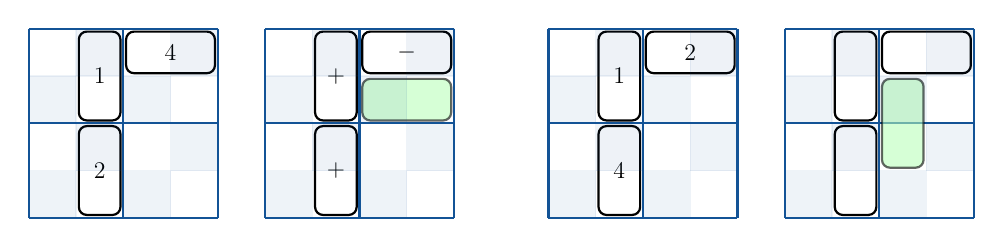
\begin{tikzpicture}[tableau, scale=.6]\gridLines{2}{2}\verticalDomino{1}{2}{1}\verticalDomino{3}{2}{2}\horizontalDomino{1}{3}{4}\fixedSquaresForGrid{2}{2}
        \gridLinesShift{2}{2}{5}
        \verticalDominoShift{1}{2}{+}{5}
        \verticalDominoShift{3}{2}{+}{5}
        \horizontalDominoShift{1}{3}{-}{5}
        \horizontalDominoRSShift{2}{3}{}{5}
        \fixedSquaresForGridShift{2}{2}{5}
        \gridLinesShift{2}{2}{11}
        \verticalDominoShift{1}{2}{1}{11}\horizontalDominoShift{1}{3}{2}{11}\verticalDominoShift{3}{2}{4}{11}\fixedSquaresForGridShift{2}{2}{11}
        \gridLinesShift{2}{2}{16}
        \verticalDominoShift{1}{2}{}{16}
        \horizontalDominoShift{1}{3}{}{16}
        \verticalDominoShift{3}{2}{}{16}
        \verticalDominoRSShift{2}{3}{}{16}
        \fixedSquaresForGridShiftAlt{2}{2}{16}
        \end{tikzpicture}
      \end{figure}
      goes to
      \begin{figure}[H]
        % 1+ 2+ 4- 3_5
        \centering
        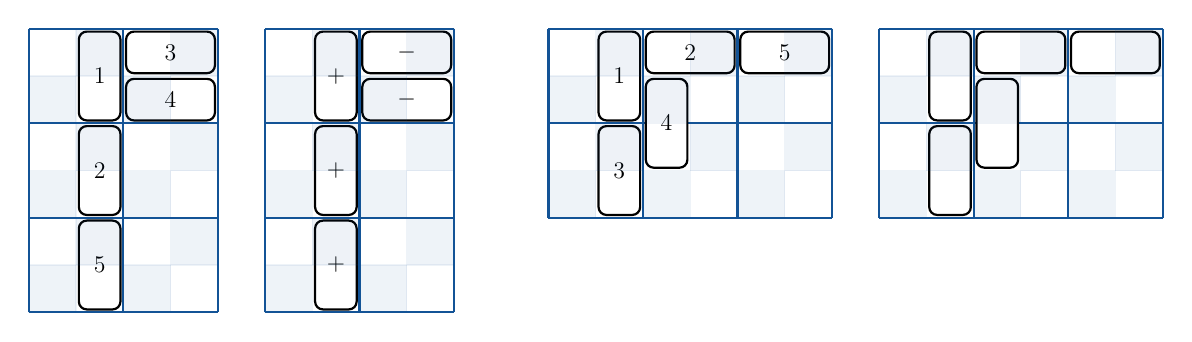
\begin{tikzpicture}[tableau, scale=.6]\gridLines{3}{2}\verticalDomino{1}{2}{1}\verticalDomino{3}{2}{2}\horizontalDomino{1}{3}{3}\horizontalDomino{2}{3}{4}\verticalDomino{5}{2}{5}\fixedSquaresForGrid{3}{2}\gridLinesShift{3}{2}{5}\verticalDominoShift{1}{2}{+}{5}\verticalDominoShift{3}{2}{+}{5}\horizontalDominoShift{1}{3}{-}{5}\horizontalDominoShift{2}{3}{-}{5}\verticalDominoShift{5}{2}{+}{5}\fixedSquaresForGridShift{3}{2}{5}\gridLinesShift{2}{3}{11}\verticalDominoShift{1}{2}{1}{11}\horizontalDominoShift{1}{3}{2}{11}\verticalDominoShift{3}{2}{3}{11}\verticalDominoShift{2}{3}{4}{11}\horizontalDominoShift{1}{5}{5}{11}\fixedSquaresForGridShift{2}{3}{11}\gridLinesShift{2}{3}{18}\verticalDominoShift{1}{2}{}{18}\horizontalDominoShift{1}{3}{}{18}\verticalDominoShift{3}{2}{}{18}\verticalDominoShift{2}{3}{}{18}\horizontalDominoShift{1}{5}{}{18}\fixedSquaresForGridShiftAlt{2}{3}{18}\end{tikzpicture}
      \end{figure}

      \item Here the corner domino has a $+$ sign, the top domino is blank (with dual sign $s$), and the column to the left has all $+$ signs.
      We give the added domino a $-$ sign and then blank it and the corner domino.
      Then we add a $+$ sign below.
      \begin{figure}[H]
        % 1+ 2+ 3s 6- 5_7
        \centering
        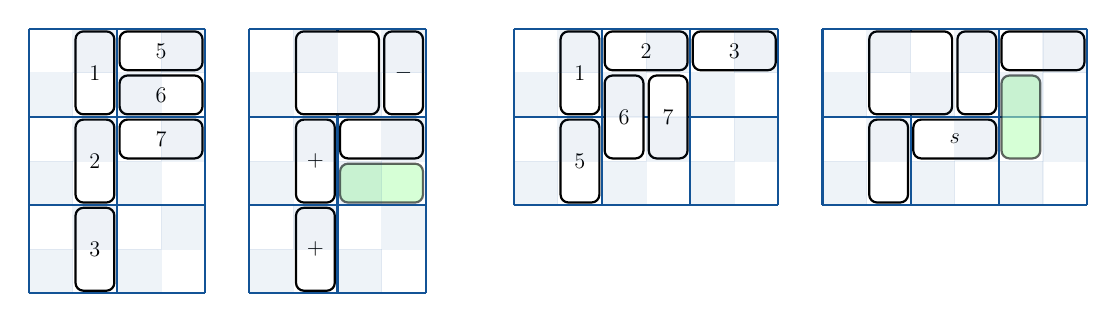
\begin{tikzpicture}[tableau, scale=.56]\gridLines{3}{2}\verticalDomino{1}{2}{1}\verticalDomino{3}{2}{2}\verticalDomino{5}{2}{3}\horizontalDomino{1}{3}{5}\horizontalDomino{2}{3}{6}\horizontalDomino{3}{3}{7}\fixedSquaresForGrid{3}{2}
        \gridLinesShift{3}{2}{5}
        \verticalDominoShift{3}{2}{+}{5}
        \verticalDominoShift{5}{2}{+}{5}
        \verticalDominoShift{1}{4}{-}{5}
        \horizontalDominoShift{3}{3}{}{5}
        \horizontalDominoRSShift{4}{3}{}{5}
        \emptyBoxShift{1}{2}{5}
        \fixedSquaresForGridShift{3}{2}{5}
        \gridLinesShift{2}{3}{11}\verticalDominoShift{1}{2}{1}{11}\horizontalDominoShift{1}{3}{2}{11}\horizontalDominoShift{1}{5}{3}{11}\verticalDominoShift{3}{2}{5}{11}\verticalDominoShift{2}{3}{6}{11}\verticalDominoShift{2}{4}{7}{11}\fixedSquaresForGridShift{2}{3}{11}
        \gridLinesShift{2}{3}{18}
        \verticalDominoShift{1}{4}{}{18}
        \horizontalDominoShift{1}{5}{}{18}
        \verticalDominoShift{3}{2}{}{18}
        \horizontalDominoShift{3}{3}{s}{18}
        \verticalDominoRSShift{2}{5}{}{18}
        \emptyBoxShift{1}{2}{18}
        \fixedSquaresForGridShiftAlt{2}{3}{18}
        \end{tikzpicture}
      \end{figure}
      goes to
      \begin{figure}[H]
        % 1+ 2+ 3s 6- 5_7 4_8
        \centering
        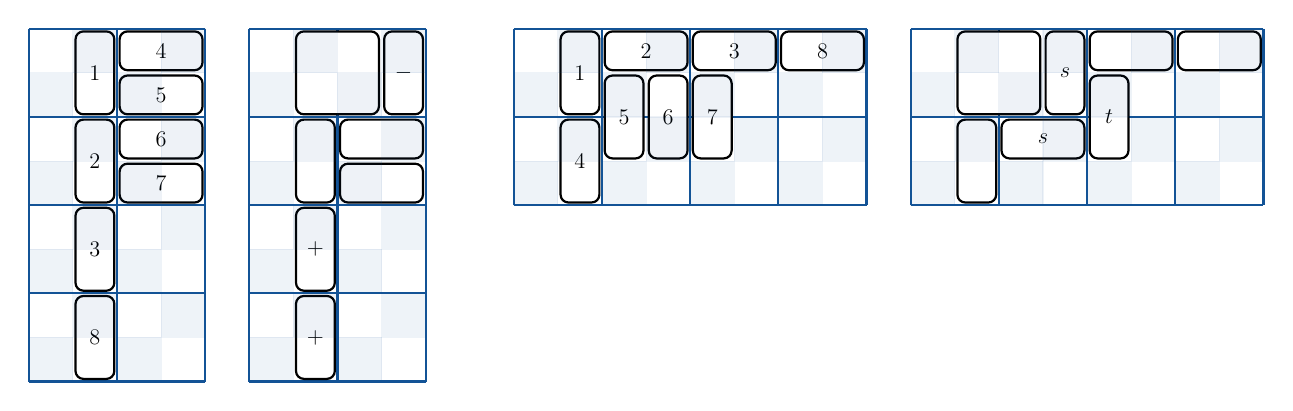
\begin{tikzpicture}[tableau, scale=.56]\gridLines{4}{2}\verticalDomino{1}{2}{1}\verticalDomino{3}{2}{2}\verticalDomino{5}{2}{3}\horizontalDomino{1}{3}{4}\horizontalDomino{2}{3}{5}\horizontalDomino{3}{3}{6}\horizontalDomino{4}{3}{7}\verticalDomino{7}{2}{8}\fixedSquaresForGrid{4}{2}\gridLinesShift{4}{2}{5}\verticalDominoShift{3}{2}{}{5}\verticalDominoShift{5}{2}{+}{5}\verticalDominoShift{1}{4}{-}{5}\horizontalDominoShift{3}{3}{}{5}\emptyBoxShift{1}{2}{5}\horizontalDominoShift{4}{3}{}{5}\verticalDominoShift{7}{2}{+}{5}\fixedSquaresForGridShift{4}{2}{5}\gridLinesShift{2}{4}{11}\verticalDominoShift{1}{2}{1}{11}\horizontalDominoShift{1}{3}{2}{11}\horizontalDominoShift{1}{5}{3}{11}\verticalDominoShift{3}{2}{4}{11}\verticalDominoShift{2}{3}{5}{11}\verticalDominoShift{2}{4}{6}{11}\verticalDominoShift{2}{5}{7}{11}\horizontalDominoShift{1}{7}{8}{11}\fixedSquaresForGridShift{2}{4}{11}\gridLinesShift{2}{4}{20}\verticalDominoShift{1}{4}{s}{20}\horizontalDominoShift{1}{5}{}{20}\verticalDominoShift{3}{2}{}{20}\horizontalDominoShift{3}{3}{s}{20}\emptyBoxShift{1}{2}{20}\verticalDominoShift{2}{5}{t}{20}\horizontalDominoShift{1}{7}{}{20}\fixedSquaresForGridShiftAlt{2}{4}{20}\end{tikzpicture}
      \end{figure}

      \item Here the corner domino has a $+$ sign, the top domino is blank (with dual sign $s$), the column to the left has a blank with an $s$ sign, and the row on top has no other signs in it.
      We'll swap the $+$ with the blank in its column, using \texttt{prepareForSign()}.
      Then we'll give the new domino a $t$ sign, and add an $s$ sign below on the dual side.
      \begin{figure}[H]
        % 1+ 3s 4s
        \centering
        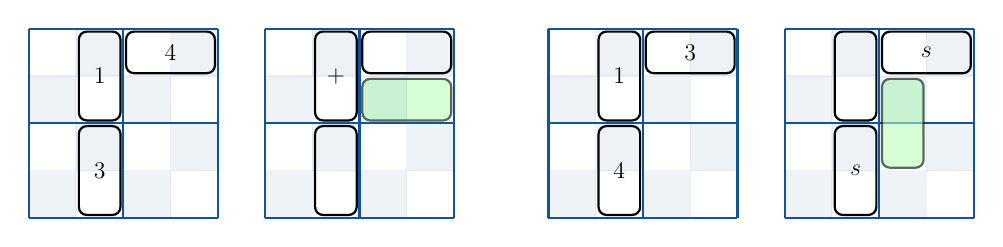
\begin{tikzpicture}[tableau, scale=.6]\gridLines{2}{2}\verticalDomino{1}{2}{1}\verticalDomino{3}{2}{3}\horizontalDomino{1}{3}{4}\fixedSquaresForGrid{2}{2}
        \gridLinesShift{2}{2}{5}\verticalDominoShift{1}{2}{+}{5}\verticalDominoShift{3}{2}{}{5}\horizontalDominoShift{1}{3}{}{5}
        \horizontalDominoRSShift{2}{3}{}{5}
        \fixedSquaresForGridShift{2}{2}{5}\gridLinesShift{2}{2}{11}\verticalDominoShift{1}{2}{1}{11}\horizontalDominoShift{1}{3}{3}{11}\verticalDominoShift{3}{2}{4}{11}\fixedSquaresForGridShift{2}{2}{11}
        \gridLinesShift{2}{2}{16}\verticalDominoShift{1}{2}{}{16}\horizontalDominoShift{1}{3}{s}{16}\verticalDominoShift{3}{2}{s}{16}
        \verticalDominoRSShift{2}{3}{}{16}
        \fixedSquaresForGridShiftAlt{2}{2}{16}\end{tikzpicture}
      \end{figure}
      goes to
      \begin{figure}[H]
        % 1+ 3s 4s
        \centering
        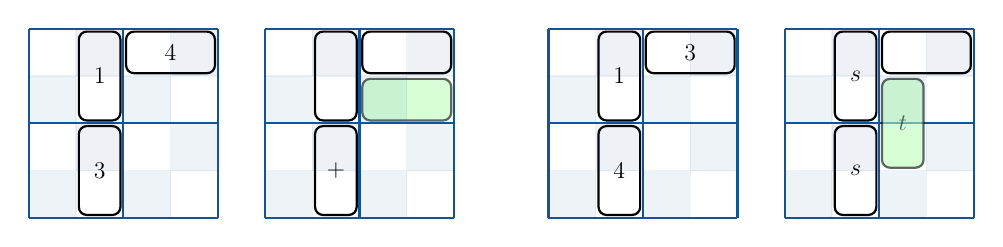
\begin{tikzpicture}[tableau, scale=.6]\gridLines{2}{2}\verticalDomino{1}{2}{1}\verticalDomino{3}{2}{3}\horizontalDomino{1}{3}{4}\fixedSquaresForGrid{2}{2}
        \gridLinesShift{2}{2}{5}
        \verticalDominoShift{1}{2}{}{5}
        \verticalDominoShift{3}{2}{+}{5}
        \horizontalDominoShift{1}{3}{}{5}
        \horizontalDominoRSShift{2}{3}{}{5}
        \fixedSquaresForGridShift{2}{2}{5}\gridLinesShift{2}{2}{11}\verticalDominoShift{1}{2}{1}{11}\horizontalDominoShift{1}{3}{3}{11}\verticalDominoShift{3}{2}{4}{11}\fixedSquaresForGridShift{2}{2}{11}
        \gridLinesShift{2}{2}{16}
        \verticalDominoShift{1}{2}{s}{16}
        \horizontalDominoShift{1}{3}{}{16}
        \verticalDominoShift{3}{2}{s}{16}
        \verticalDominoRSShift{2}{3}{t}{16}
        \fixedSquaresForGridShiftAlt{2}{2}{16}\end{tikzpicture}
      \end{figure}
      goes to
      \begin{figure}[H]
        % 1+ 3s 4s 2_5
        \centering
        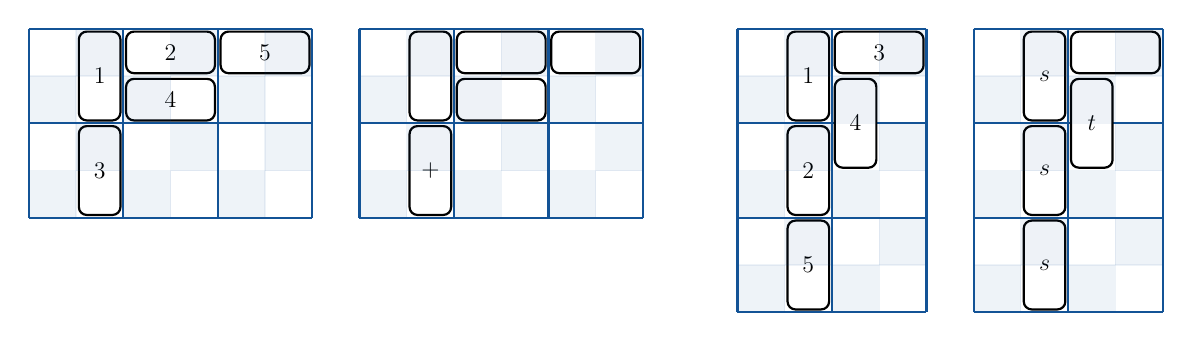
\begin{tikzpicture}[tableau, scale=.6]\gridLines{2}{3}\verticalDomino{1}{2}{1}\horizontalDomino{1}{3}{2}\verticalDomino{3}{2}{3}\horizontalDomino{2}{3}{4}\horizontalDomino{1}{5}{5}\fixedSquaresForGrid{2}{3}\gridLinesShift{2}{3}{7}\verticalDominoShift{1}{2}{}{7}\verticalDominoShift{3}{2}{+}{7}\horizontalDominoShift{1}{3}{}{7}\horizontalDominoShift{2}{3}{}{7}\horizontalDominoShift{1}{5}{}{7}\fixedSquaresForGridShift{2}{3}{7}\gridLinesShift{3}{2}{15}\verticalDominoShift{1}{2}{1}{15}\verticalDominoShift{3}{2}{2}{15}\horizontalDominoShift{1}{3}{3}{15}\verticalDominoShift{2}{3}{4}{15}\verticalDominoShift{5}{2}{5}{15}\fixedSquaresForGridShift{3}{2}{15}\gridLinesShift{3}{2}{20}\verticalDominoShift{1}{2}{s}{20}\horizontalDominoShift{1}{3}{}{20}\verticalDominoShift{3}{2}{s}{20}\verticalDominoShift{2}{3}{t}{20}\verticalDominoShift{5}{2}{s}{20}\fixedSquaresForGridShiftAlt{3}{2}{20}\end{tikzpicture}
      \end{figure}

      \item Here the corner domino is blank, there is a ($+$) sign in the top row, and all the dominoes in the column below the corner domino contain $+$ signs.
      We'll swap the signed domino with the corner domino, using \texttt{prepareForSign()} on the dual side.
      Then we'll proceed as in two cases ago.
      \begin{figure}[H]
        % 1+ 2s 4+
        \centering
        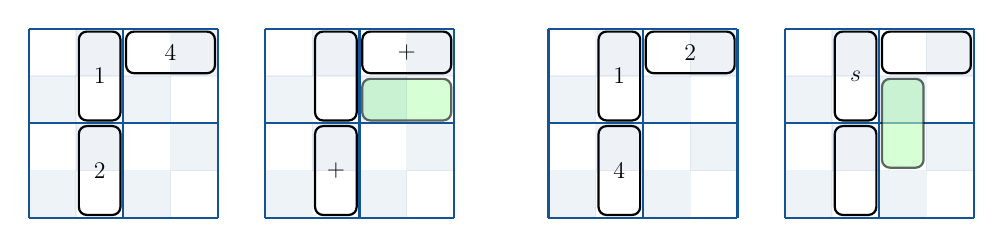
\begin{tikzpicture}[tableau, scale=.6]\gridLines{2}{2}\verticalDomino{1}{2}{1}\verticalDomino{3}{2}{2}\horizontalDomino{1}{3}{4}\fixedSquaresForGrid{2}{2}
        \gridLinesShift{2}{2}{5}
        \verticalDominoShift{1}{2}{}{5}
        \verticalDominoShift{3}{2}{+}{5}
        \horizontalDominoShift{1}{3}{+}{5}
        \horizontalDominoRSShift{2}{3}{}{5}
        \fixedSquaresForGridShift{2}{2}{5}
        \gridLinesShift{2}{2}{11}\verticalDominoShift{1}{2}{1}{11}\horizontalDominoShift{1}{3}{2}{11}\verticalDominoShift{3}{2}{4}{11}\fixedSquaresForGridShift{2}{2}{11}
        \gridLinesShift{2}{2}{16}
        \verticalDominoShift{1}{2}{s}{16}
        \horizontalDominoShift{1}{3}{}{16}
        \verticalDominoShift{3}{2}{}{16}
        \verticalDominoRSShift{2}{3}{}{16}
        \fixedSquaresForGridShiftAlt{2}{2}{16}
        \end{tikzpicture}
      \end{figure}
      goes to
      \begin{figure}[H]
        % 1+ 2s 4+
        \centering
        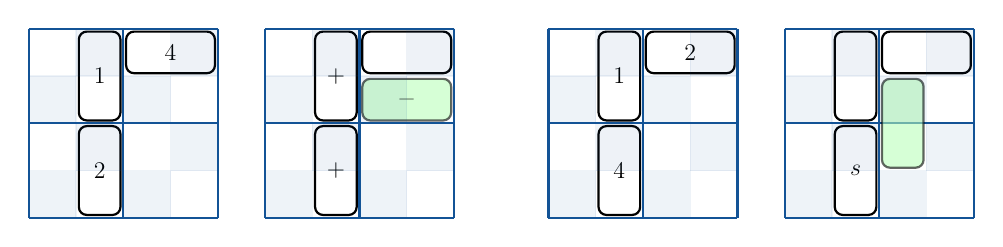
\begin{tikzpicture}[tableau, scale=.6]\gridLines{2}{2}\verticalDomino{1}{2}{1}\verticalDomino{3}{2}{2}\horizontalDomino{1}{3}{4}\fixedSquaresForGrid{2}{2}
        \gridLinesShift{2}{2}{5}
        \verticalDominoShift{1}{2}{+}{5}
        \verticalDominoShift{3}{2}{+}{5}
        \horizontalDominoShift{1}{3}{}{5}
        \horizontalDominoRSShift{2}{3}{-}{5}
        \fixedSquaresForGridShift{2}{2}{5}
        \gridLinesShift{2}{2}{11}\verticalDominoShift{1}{2}{1}{11}\horizontalDominoShift{1}{3}{2}{11}\verticalDominoShift{3}{2}{4}{11}\fixedSquaresForGridShift{2}{2}{11}
        \gridLinesShift{2}{2}{16}
        \verticalDominoShift{1}{2}{}{16}
        \horizontalDominoShift{1}{3}{}{16}
        \verticalDominoShift{3}{2}{s}{16}
        \verticalDominoRSShift{2}{3}{}{16}
        \fixedSquaresForGridShiftAlt{2}{2}{16}
        \end{tikzpicture}
      \end{figure}
      goes to
      \begin{figure}[H]
        % 1+ 2s 4+
        \centering
        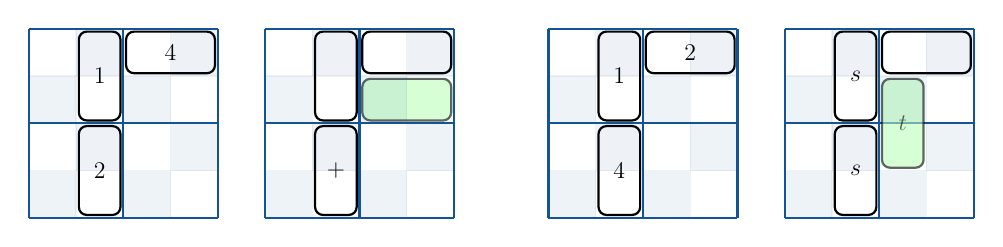
\begin{tikzpicture}[tableau, scale=.6]\gridLines{2}{2}\verticalDomino{1}{2}{1}\verticalDomino{3}{2}{2}\horizontalDomino{1}{3}{4}\fixedSquaresForGrid{2}{2}
        \gridLinesShift{2}{2}{5}
        \verticalDominoShift{1}{2}{}{5}
        \verticalDominoShift{3}{2}{+}{5}
        \horizontalDominoShift{1}{3}{}{5}
        \horizontalDominoRSShift{2}{3}{}{5}
        \fixedSquaresForGridShift{2}{2}{5}
        \gridLinesShift{2}{2}{11}\verticalDominoShift{1}{2}{1}{11}\horizontalDominoShift{1}{3}{2}{11}\verticalDominoShift{3}{2}{4}{11}\fixedSquaresForGridShift{2}{2}{11}
        \gridLinesShift{2}{2}{16}
        \verticalDominoShift{1}{2}{s}{16}
        \horizontalDominoShift{1}{3}{}{16}
        \verticalDominoShift{3}{2}{s}{16}
        \verticalDominoRSShift{2}{3}{t}{16}
        \fixedSquaresForGridShiftAlt{2}{2}{16}
        \end{tikzpicture}
      \end{figure}
      goes to
      \begin{figure}[H]
        % 1+ 2s 4+ 3_5
        \centering
        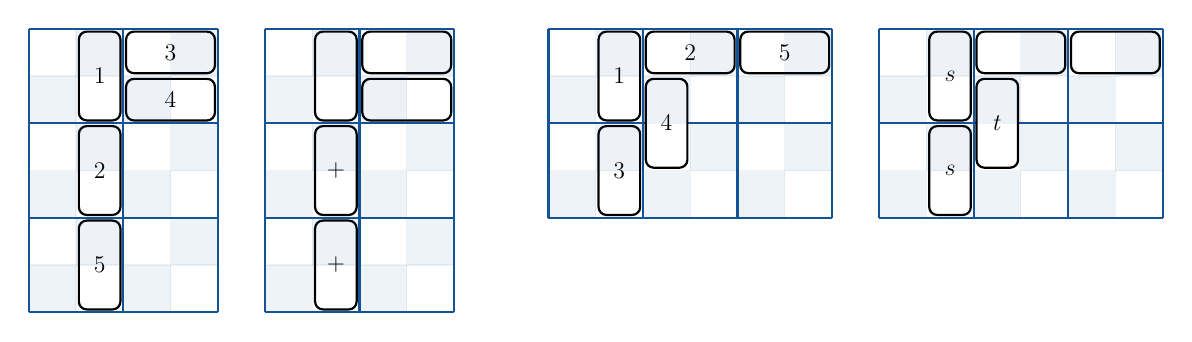
\begin{tikzpicture}[tableau, scale=.6]\gridLines{3}{2}\verticalDomino{1}{2}{1}\verticalDomino{3}{2}{2}\horizontalDomino{1}{3}{3}\horizontalDomino{2}{3}{4}\verticalDomino{5}{2}{5}\fixedSquaresForGrid{3}{2}\gridLinesShift{3}{2}{5}\verticalDominoShift{1}{2}{}{5}\verticalDominoShift{3}{2}{+}{5}\horizontalDominoShift{1}{3}{}{5}\horizontalDominoShift{2}{3}{}{5}\verticalDominoShift{5}{2}{+}{5}\fixedSquaresForGridShift{3}{2}{5}\gridLinesShift{2}{3}{11}\verticalDominoShift{1}{2}{1}{11}\horizontalDominoShift{1}{3}{2}{11}\verticalDominoShift{3}{2}{3}{11}\verticalDominoShift{2}{3}{4}{11}\horizontalDominoShift{1}{5}{5}{11}\fixedSquaresForGridShift{2}{3}{11}\gridLinesShift{2}{3}{18}\verticalDominoShift{1}{2}{s}{18}\horizontalDominoShift{1}{3}{}{18}\verticalDominoShift{3}{2}{s}{18}\verticalDominoShift{2}{3}{t}{18}\horizontalDominoShift{1}{5}{}{18}\fixedSquaresForGridShiftAlt{2}{3}{18}\end{tikzpicture}
      \end{figure}

      \item Here there is no sign in the top row.
      In this case, on the dual side, the column is filled with ($s$) signs.
      We give the new domino a $t$ and go down with an $s$ on the dual side.
      \begin{figure}[H]
        % 1s 2_-4
        \centering
        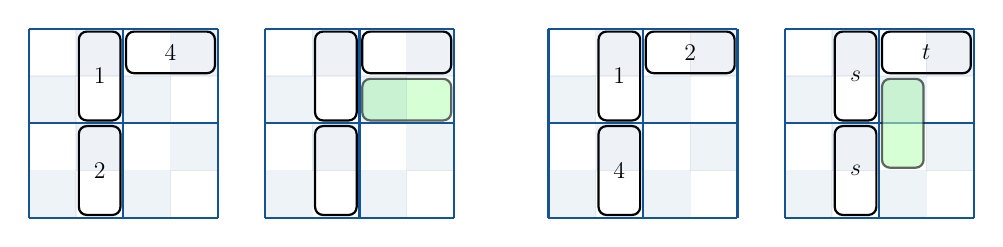
\begin{tikzpicture}[tableau, scale=.6]\gridLines{2}{2}\verticalDomino{1}{2}{1}\verticalDomino{3}{2}{2}\horizontalDomino{1}{3}{4}\fixedSquaresForGrid{2}{2}
        \gridLinesShift{2}{2}{5}
        \verticalDominoShift{1}{2}{}{5}
        \verticalDominoShift{3}{2}{}{5}
        \horizontalDominoShift{1}{3}{}{5}
        \horizontalDominoRSShift{2}{3}{}{5}
        \fixedSquaresForGridShift{2}{2}{5}
        \gridLinesShift{2}{2}{11}\verticalDominoShift{1}{2}{1}{11}\horizontalDominoShift{1}{3}{2}{11}\verticalDominoShift{3}{2}{4}{11}\fixedSquaresForGridShift{2}{2}{11}
        \gridLinesShift{2}{2}{16}
        \verticalDominoShift{1}{2}{s}{16}
        \horizontalDominoShift{1}{3}{t}{16}
        \verticalDominoShift{3}{2}{s}{16}
        \verticalDominoRSShift{2}{3}{}{16}
        \fixedSquaresForGridShiftAlt{2}{2}{16}
        \end{tikzpicture}
      \end{figure}
      goes to
      \begin{figure}[H]
        % 1s 2_-4 3_5
        \centering
        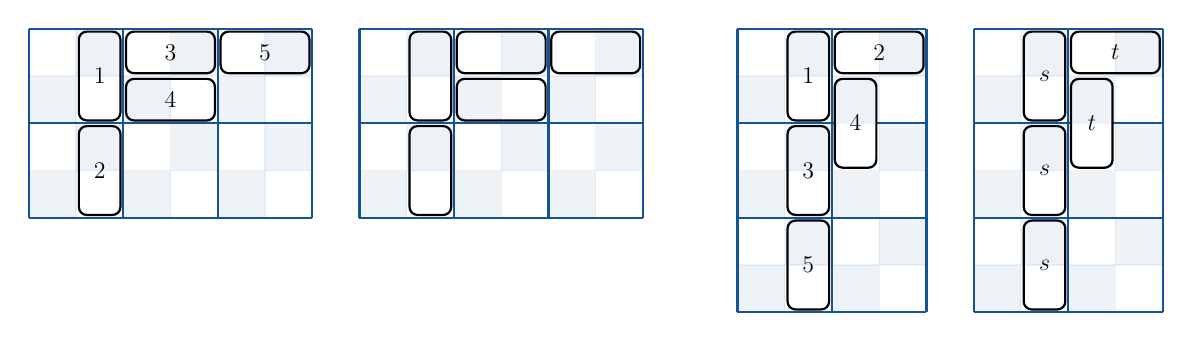
\begin{tikzpicture}[tableau, scale=.6]\gridLines{2}{3}\verticalDomino{1}{2}{1}\verticalDomino{3}{2}{2}\horizontalDomino{1}{3}{3}\horizontalDomino{2}{3}{4}\horizontalDomino{1}{5}{5}\fixedSquaresForGrid{2}{3}\gridLinesShift{2}{3}{7}\verticalDominoShift{1}{2}{}{7}\verticalDominoShift{3}{2}{}{7}\horizontalDominoShift{1}{3}{}{7}\horizontalDominoShift{2}{3}{}{7}\horizontalDominoShift{1}{5}{}{7}\fixedSquaresForGridShift{2}{3}{7}\gridLinesShift{3}{2}{15}\verticalDominoShift{1}{2}{1}{15}\horizontalDominoShift{1}{3}{2}{15}\verticalDominoShift{3}{2}{3}{15}\verticalDominoShift{2}{3}{4}{15}\verticalDominoShift{5}{2}{5}{15}\fixedSquaresForGridShift{3}{2}{15}\gridLinesShift{3}{2}{20}\verticalDominoShift{1}{2}{s}{20}\horizontalDominoShift{1}{3}{t}{20}\verticalDominoShift{3}{2}{s}{20}\verticalDominoShift{2}{3}{t}{20}\verticalDominoShift{5}{2}{s}{20}\fixedSquaresForGridShiftAlt{3}{2}{20}\end{tikzpicture}
      \end{figure}
      Here is another example.  (The column need not be all blanks.)
      \begin{figure}[H]
        % 1s 4- 2_-5 3_7
        \centering
        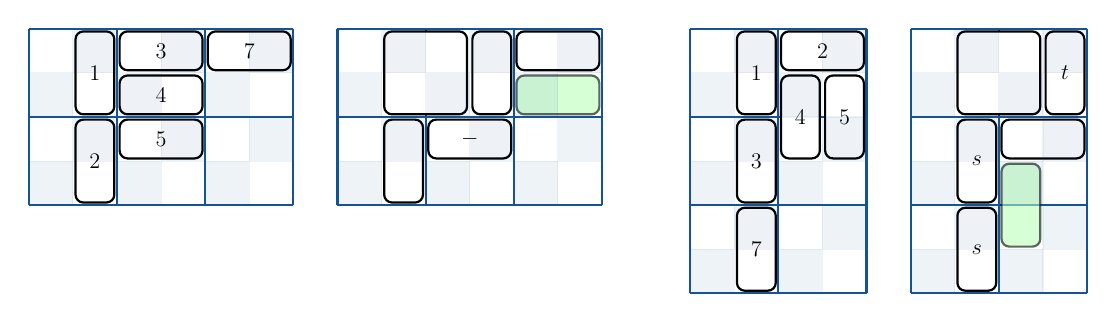
\begin{tikzpicture}[tableau, scale=.56]\gridLines{2}{3}\verticalDomino{1}{2}{1}\verticalDomino{3}{2}{2}\horizontalDomino{1}{3}{3}\horizontalDomino{2}{3}{4}\horizontalDomino{3}{3}{5}\horizontalDomino{1}{5}{7}\fixedSquaresForGrid{2}{3}
        \gridLinesShift{2}{3}{7}
        \verticalDominoShift{1}{4}{}{7}
        \verticalDominoShift{3}{2}{}{7}
        \horizontalDominoShift{3}{3}{-}{7}
        \emptyBoxShift{1}{2}{7}
        \horizontalDominoShift{1}{5}{}{7}
        \horizontalDominoRSShift{2}{5}{}{7}
        \fixedSquaresForGridShift{2}{3}{7}
        \gridLinesShift{3}{2}{15}\verticalDominoShift{1}{2}{1}{15}\horizontalDominoShift{1}{3}{2}{15}\verticalDominoShift{3}{2}{3}{15}\verticalDominoShift{2}{3}{4}{15}\verticalDominoShift{2}{4}{5}{15}\verticalDominoShift{5}{2}{7}{15}\fixedSquaresForGridShift{3}{2}{15}
        \gridLinesShift{3}{2}{20}
        \verticalDominoShift{3}{2}{s}{20}
        \verticalDominoShift{1}{4}{t}{20}
        \horizontalDominoShift{3}{3}{}{20}
        \emptyBoxShift{1}{2}{20}
        \verticalDominoShift{5}{2}{s}{20}
        \verticalDominoRSShift{4}{3}{}{20}
        \fixedSquaresForGridShiftAlt{3}{2}{20}
        \end{tikzpicture}
      \end{figure}
      goes to
      \begin{figure}[H]
        % 1s 4- 2_-5 3_7 6_8
        \centering
        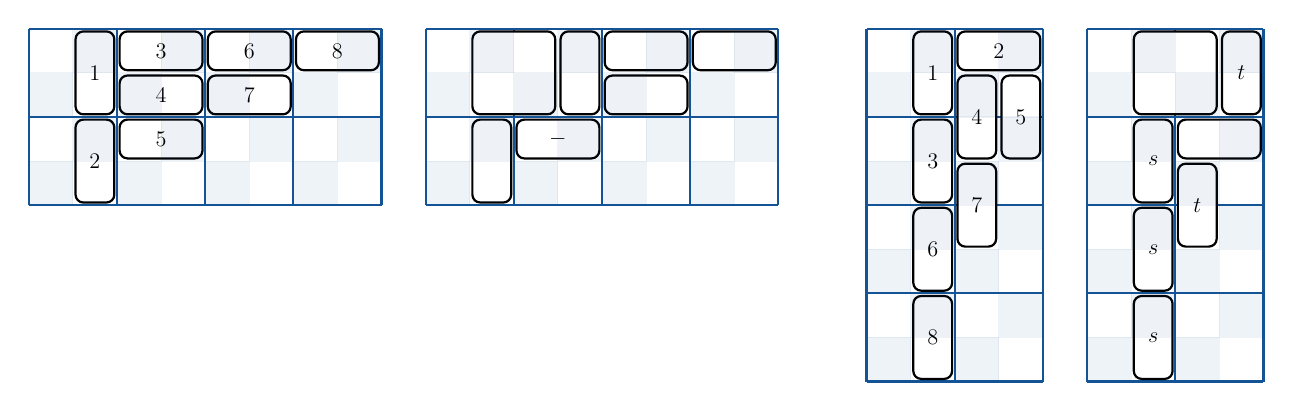
\begin{tikzpicture}[tableau, scale=.56]\gridLines{2}{4}\verticalDomino{1}{2}{1}\verticalDomino{3}{2}{2}\horizontalDomino{1}{3}{3}\horizontalDomino{2}{3}{4}\horizontalDomino{3}{3}{5}\horizontalDomino{1}{5}{6}\horizontalDomino{2}{5}{7}\horizontalDomino{1}{7}{8}\fixedSquaresForGrid{2}{4}\gridLinesShift{2}{4}{9}\verticalDominoShift{1}{4}{}{9}\verticalDominoShift{3}{2}{}{9}\horizontalDominoShift{3}{3}{-}{9}\emptyBoxShift{1}{2}{9}\horizontalDominoShift{1}{5}{}{9}\horizontalDominoShift{2}{5}{}{9}\horizontalDominoShift{1}{7}{}{9}\fixedSquaresForGridShift{2}{4}{9}\gridLinesShift{4}{2}{19}\verticalDominoShift{1}{2}{1}{19}\horizontalDominoShift{1}{3}{2}{19}\verticalDominoShift{3}{2}{3}{19}\verticalDominoShift{2}{3}{4}{19}\verticalDominoShift{2}{4}{5}{19}\verticalDominoShift{5}{2}{6}{19}\verticalDominoShift{4}{3}{7}{19}\verticalDominoShift{7}{2}{8}{19}\fixedSquaresForGridShift{4}{2}{19}\gridLinesShift{4}{2}{24}\verticalDominoShift{3}{2}{s}{24}\verticalDominoShift{1}{4}{t}{24}\horizontalDominoShift{3}{3}{}{24}\emptyBoxShift{1}{2}{24}\verticalDominoShift{5}{2}{s}{24}\verticalDominoShift{4}{3}{t}{24}\verticalDominoShift{7}{2}{s}{24}\fixedSquaresForGridShiftAlt{4}{2}{24}\end{tikzpicture}
      \end{figure}
    \end{itemize}

    There still remains the cases where we break a cycle and don't close it again.
    They parallel the cases listed above.
    We also need to include the adjustments which we made in the other list of cases, for when there is a relevant shape change.

    \item Here $gpos = W$ and $dgpos = X$ and \pos\ is horizontal and \dpos\ is vertical.
    Here we are extending an unboxed cycle.
    With $(x, y)$ the coordinates of the square in grid position $W$, the pair domino occupies $(x - 1, y - 1)$.
    The pair domino is the top of the cycle which we are adjacent to.
    There are several cases.
    \begin{itemize}
      \item Here the pair domino is blank (with $s$ on the dual side), and there is a ($+$) sign in the row of the pair domino.
      Here we just swap the blank with the $+$ sign (using \texttt{prepareForSign()} on the dual side), and give the new domino a $-$ sign.
      Then we adjust the signs in the new domino and the pair domino (and their duals if necessary) to match the cycle which we are joining.
      Then we add a $+$ sign below.
      Here is an example.
      \begin{figure}[H]
        % 1s 2+ 3_-4 6+
        \centering
        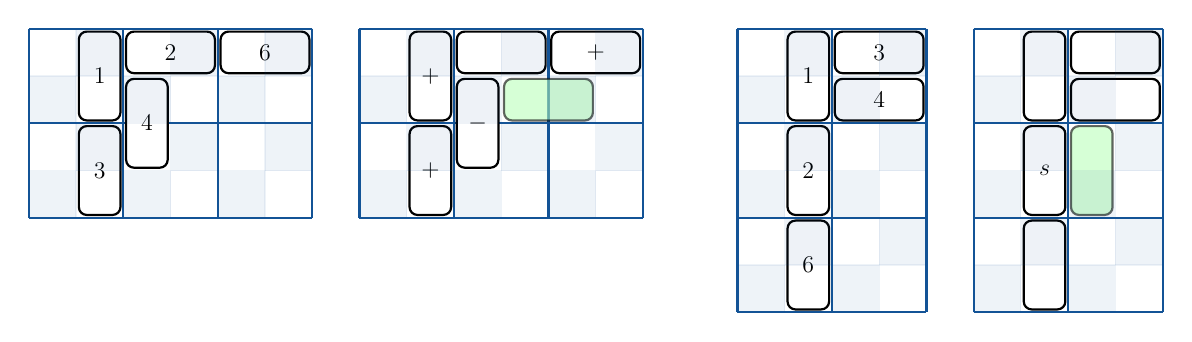
\begin{tikzpicture}[tableau, scale=.6]\gridLines{2}{3}\verticalDomino{1}{2}{1}\horizontalDomino{1}{3}{2}\verticalDomino{3}{2}{3}\verticalDomino{2}{3}{4}\horizontalDomino{1}{5}{6}\fixedSquaresForGrid{2}{3}
        \gridLinesShift{2}{3}{7}\verticalDominoShift{1}{2}{+}{7}\horizontalDominoShift{1}{3}{}{7}\verticalDominoShift{3}{2}{+}{7}\verticalDominoShift{2}{3}{-}{7}\horizontalDominoShift{1}{5}{+}{7}
        \horizontalDominoRSShift{2}{4}{}{7}
        \fixedSquaresForGridShift{2}{3}{7}
        \gridLinesShift{3}{2}{15}\verticalDominoShift{1}{2}{1}{15}\verticalDominoShift{3}{2}{2}{15}\horizontalDominoShift{1}{3}{3}{15}\horizontalDominoShift{2}{3}{4}{15}\verticalDominoShift{5}{2}{6}{15}\fixedSquaresForGridShift{3}{2}{15}
        \gridLinesShift{3}{2}{20}\verticalDominoShift{1}{2}{}{20}\verticalDominoShift{3}{2}{s}{20}\horizontalDominoShift{1}{3}{}{20}\horizontalDominoShift{2}{3}{}{20}
        \verticalDominoRSShift{3}{3}{}{20}
        \verticalDominoShift{5}{2}{}{20}\fixedSquaresForGridShiftAlt{3}{2}{20}\end{tikzpicture}
      \end{figure}
      goes to
      \begin{figure}[H]
        % 1s 2+ 3_-4 6+ 5_7
        \centering
        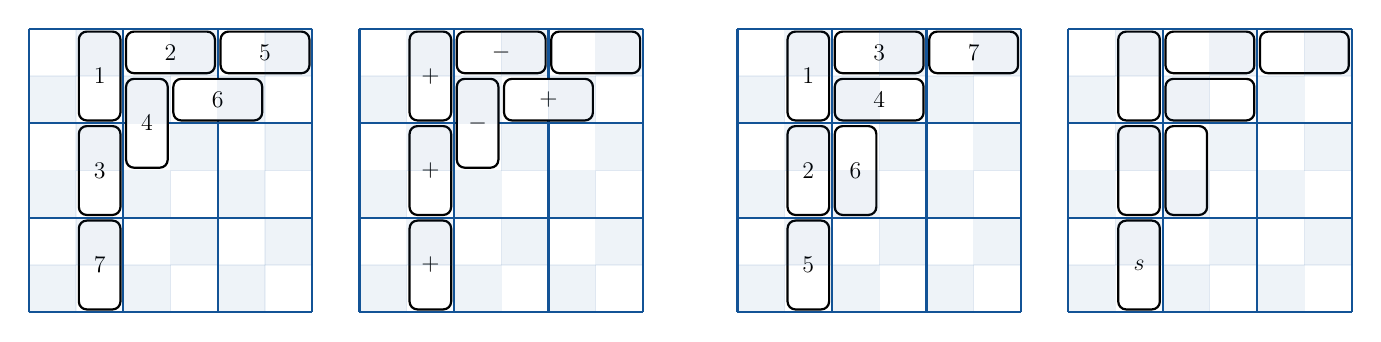
\begin{tikzpicture}[tableau, scale=.6]\gridLines{3}{3}\verticalDomino{1}{2}{1}\horizontalDomino{1}{3}{2}\verticalDomino{3}{2}{3}\verticalDomino{2}{3}{4}\horizontalDomino{1}{5}{5}\horizontalDomino{2}{4}{6}\verticalDomino{5}{2}{7}\fixedSquaresForGrid{3}{3}\gridLinesShift{3}{3}{7}\verticalDominoShift{1}{2}{+}{7}\horizontalDominoShift{1}{3}{-}{7}\verticalDominoShift{3}{2}{+}{7}\verticalDominoShift{2}{3}{-}{7}\horizontalDominoShift{1}{5}{}{7}\horizontalDominoShift{2}{4}{+}{7}\verticalDominoShift{5}{2}{+}{7}\fixedSquaresForGridShift{3}{3}{7}\gridLinesShift{3}{3}{15}\verticalDominoShift{1}{2}{1}{15}\verticalDominoShift{3}{2}{2}{15}\horizontalDominoShift{1}{3}{3}{15}\horizontalDominoShift{2}{3}{4}{15}\verticalDominoShift{5}{2}{5}{15}\verticalDominoShift{3}{3}{6}{15}\horizontalDominoShift{1}{5}{7}{15}\fixedSquaresForGridShift{3}{3}{15}\gridLinesShift{3}{3}{22}\verticalDominoShift{1}{2}{}{22}\verticalDominoShift{3}{2}{}{22}\horizontalDominoShift{1}{3}{}{22}\horizontalDominoShift{2}{3}{}{22}\verticalDominoShift{5}{2}{s}{22}\verticalDominoShift{3}{3}{}{22}\horizontalDominoShift{1}{5}{}{22}\fixedSquaresForGridShiftAlt{3}{3}{22}\end{tikzpicture}
      \end{figure}

      \item Here the pair domino has a ($+$) sign.
      We give the new domino a $-$ sign, and then adjust the pair domino and new domino signs to conform to what's already in the cycle.
      If the domino to the right of the pair domino has a $-$, we're done (except for adding a $+$ sign below).
      \begin{figure}[H]
        % 1s 2+ 3t 4t 6-
        \centering
        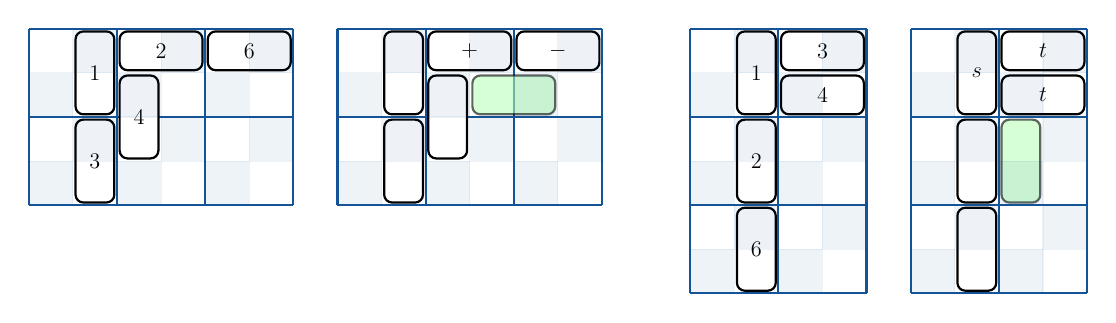
\begin{tikzpicture}[tableau, scale=.56]\gridLines{2}{3}\verticalDomino{1}{2}{1}\horizontalDomino{1}{3}{2}\verticalDomino{3}{2}{3}\verticalDomino{2}{3}{4}\horizontalDomino{1}{5}{6}\fixedSquaresForGrid{2}{3}
        \gridLinesShift{2}{3}{7}\verticalDominoShift{1}{2}{}{7}\horizontalDominoShift{1}{3}{+}{7}\verticalDominoShift{3}{2}{}{7}\verticalDominoShift{2}{3}{}{7}\horizontalDominoShift{1}{5}{-}{7}
        \horizontalDominoRSShift{2}{4}{}{7}
        \fixedSquaresForGridShift{2}{3}{7}
        \gridLinesShift{3}{2}{15}\verticalDominoShift{1}{2}{1}{15}\verticalDominoShift{3}{2}{2}{15}\horizontalDominoShift{1}{3}{3}{15}\horizontalDominoShift{2}{3}{4}{15}\verticalDominoShift{5}{2}{6}{15}\fixedSquaresForGridShift{3}{2}{15}
        \gridLinesShift{3}{2}{20}\verticalDominoShift{1}{2}{s}{20}\verticalDominoShift{3}{2}{}{20}\horizontalDominoShift{1}{3}{t}{20}\horizontalDominoShift{2}{3}{t}{20}\verticalDominoShift{5}{2}{}{20}
        \verticalDominoRSShift{3}{3}{}{20}
        \fixedSquaresForGridShiftAlt{3}{2}{20}\end{tikzpicture}
      \end{figure}
      goes to
      \begin{figure}[H]
        % 1s 2+ 3t 4t 6-
        \centering
        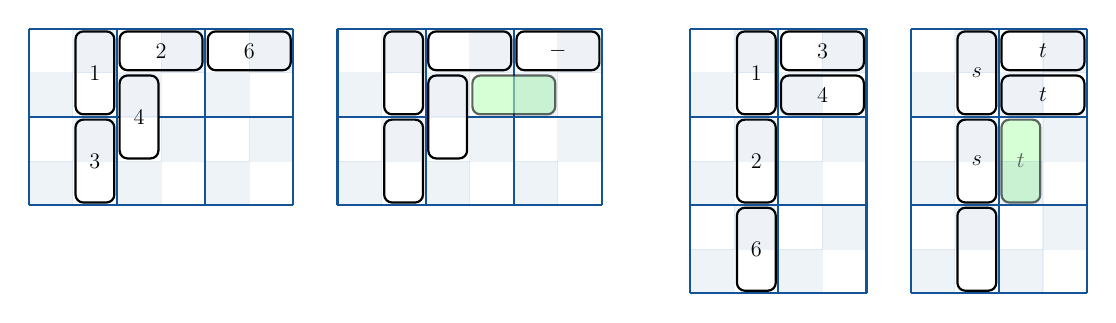
\begin{tikzpicture}[tableau, scale=.56]\gridLines{2}{3}\verticalDomino{1}{2}{1}\horizontalDomino{1}{3}{2}\verticalDomino{3}{2}{3}\verticalDomino{2}{3}{4}\horizontalDomino{1}{5}{6}\fixedSquaresForGrid{2}{3}
        \gridLinesShift{2}{3}{7}\verticalDominoShift{1}{2}{}{7}\horizontalDominoShift{1}{3}{}{7}\verticalDominoShift{3}{2}{}{7}\verticalDominoShift{2}{3}{}{7}\horizontalDominoShift{1}{5}{-}{7}
        \horizontalDominoRSShift{2}{4}{}{7}
        \fixedSquaresForGridShift{2}{3}{7}
        \gridLinesShift{3}{2}{15}\verticalDominoShift{1}{2}{1}{15}\verticalDominoShift{3}{2}{2}{15}\horizontalDominoShift{1}{3}{3}{15}\horizontalDominoShift{2}{3}{4}{15}\verticalDominoShift{5}{2}{6}{15}\fixedSquaresForGridShift{3}{2}{15}
        \gridLinesShift{3}{2}{20}\verticalDominoShift{1}{2}{s}{20}\verticalDominoShift{3}{2}{s}{20}\horizontalDominoShift{1}{3}{t}{20}\horizontalDominoShift{2}{3}{t}{20}\verticalDominoShift{5}{2}{}{20}
        \verticalDominoRSShift{3}{3}{t}{20}
        \fixedSquaresForGridShiftAlt{3}{2}{20}\end{tikzpicture}
      \end{figure}
      goes to
      \begin{figure}[H]
        % 1s 2+ 3t 4t 6- 5_7
        \centering
        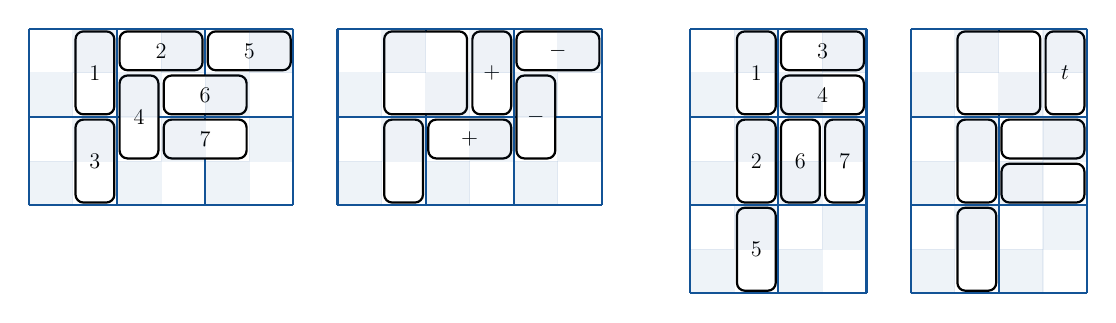
\begin{tikzpicture}[tableau, scale=.56]\gridLines{2}{3}\verticalDomino{1}{2}{1}\horizontalDomino{1}{3}{2}\verticalDomino{3}{2}{3}\verticalDomino{2}{3}{4}\horizontalDomino{1}{5}{5}\horizontalDomino{2}{4}{6}\horizontalDomino{3}{4}{7}\fixedSquaresForGrid{2}{3}\gridLinesShift{2}{3}{7}\verticalDominoShift{1}{4}{+}{7}\verticalDominoShift{3}{2}{}{7}\horizontalDominoShift{1}{5}{-}{7}\verticalDominoShift{2}{5}{-}{7}\horizontalDominoShift{3}{3}{+}{7}\emptyBoxShift{1}{2}{7}\fixedSquaresForGridShift{2}{3}{7}\gridLinesShift{3}{2}{15}\verticalDominoShift{1}{2}{1}{15}\verticalDominoShift{3}{2}{2}{15}\horizontalDominoShift{1}{3}{3}{15}\horizontalDominoShift{2}{3}{4}{15}\verticalDominoShift{5}{2}{5}{15}\verticalDominoShift{3}{3}{6}{15}\verticalDominoShift{3}{4}{7}{15}\fixedSquaresForGridShift{3}{2}{15}\gridLinesShift{3}{2}{20}\verticalDominoShift{3}{2}{}{20}\verticalDominoShift{1}{4}{t}{20}\verticalDominoShift{5}{2}{}{20}\horizontalDominoShift{4}{3}{}{20}\horizontalDominoShift{3}{3}{}{20}\emptyBoxShift{1}{2}{20}\fixedSquaresForGridShiftAlt{3}{2}{20}\end{tikzpicture}
      \end{figure}

      If instead the domino to the right of the pair domino is blank, we need to put that sign (on the dual side) into the cycle.
      We do this as if first placing the sign in the bottom of the old cycle, and then extending this cycle by one pair.
      Note that since we are placing the sign into a boxed cycle, there will not be a shape change.
      \begin{figure}[H]
        % 1s 2t 3s 5+ 4_6 7s 10- 9_11
        \centering
        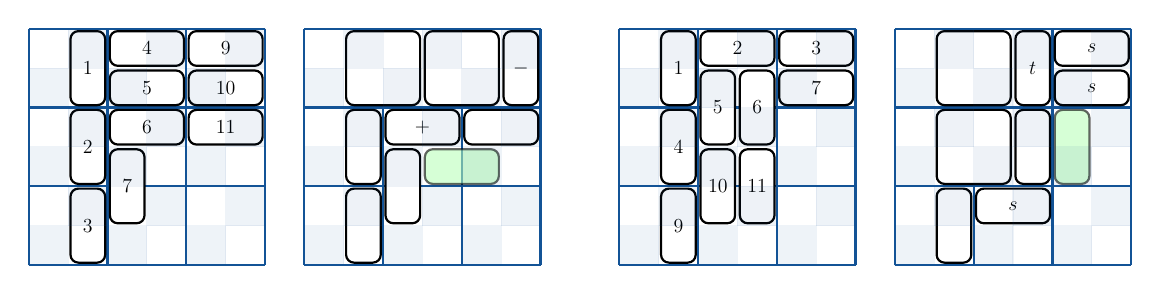
\begin{tikzpicture}[tableau, scale=.5]\gridLines{3}{3}\verticalDomino{1}{2}{1}\verticalDomino{3}{2}{2}\verticalDomino{5}{2}{3}\horizontalDomino{1}{3}{4}\horizontalDomino{2}{3}{5}\horizontalDomino{3}{3}{6}\verticalDomino{4}{3}{7}\horizontalDomino{1}{5}{9}\horizontalDomino{2}{5}{10}\horizontalDomino{3}{5}{11}\fixedSquaresForGrid{3}{3}
        \gridLinesShift{3}{3}{7}
        \verticalDominoShift{3}{2}{}{7}
        \verticalDominoShift{5}{2}{}{7}
        \horizontalDominoShift{3}{3}{+}{7}
        \emptyBoxShift{1}{2}{7}
        \verticalDominoShift{4}{3}{}{7}
        \verticalDominoShift{1}{6}{-}{7}
        \horizontalDominoShift{3}{5}{}{7}
        \emptyBoxShift{1}{4}{7}
        \horizontalDominoRSShift{4}{4}{}{7}
        \fixedSquaresForGridShift{3}{3}{7}
        \gridLinesShift{3}{3}{15}\verticalDominoShift{1}{2}{1}{15}\horizontalDominoShift{1}{3}{2}{15}\horizontalDominoShift{1}{5}{3}{15}\verticalDominoShift{3}{2}{4}{15}\verticalDominoShift{2}{3}{5}{15}\verticalDominoShift{2}{4}{6}{15}\horizontalDominoShift{2}{5}{7}{15}\verticalDominoShift{5}{2}{9}{15}\verticalDominoShift{4}{3}{10}{15}\verticalDominoShift{4}{4}{11}{15}\fixedSquaresForGridShift{3}{3}{15}
        \gridLinesShift{3}{3}{22}
        \verticalDominoShift{1}{4}{t}{22}
        \horizontalDominoShift{1}{5}{s}{22}
        \verticalDominoShift{3}{4}{}{22}
        \emptyBoxShift{1}{2}{22}
        \horizontalDominoShift{2}{5}{s}{22}
        \verticalDominoShift{5}{2}{}{22}
        \horizontalDominoShift{5}{3}{s}{22}
        \emptyBoxShift{3}{2}{22}
        \verticalDominoRSShift{3}{5}{}{22}
        \fixedSquaresForGridShiftAlt{3}{3}{22}
        \end{tikzpicture}
      \end{figure}
      % goes to
      % \begin{figure}[H]
      %   % 1s 2t 3s 5+ 4_6 7s 10- 9_11
      %   \centering
      %   \begin{tikzpicture}[tableau, scale=.5]\gridLines{3}{3}\verticalDomino{1}{2}{1}\verticalDomino{3}{2}{2}\verticalDomino{5}{2}{3}\horizontalDomino{1}{3}{4}\horizontalDomino{2}{3}{5}\horizontalDomino{3}{3}{6}\verticalDomino{4}{3}{7}\horizontalDomino{1}{5}{9}\horizontalDomino{2}{5}{10}\horizontalDomino{3}{5}{11}\fixedSquaresForGrid{3}{3}
      %   \gridLinesShift{3}{3}{7}
      %   \verticalDominoShift{3}{2}{}{7}
      %   \verticalDominoShift{5}{2}{}{7}
      %   \horizontalDominoShift{3}{3}{}{7}
      %   \emptyBoxShift{1}{2}{7}
      %   \verticalDominoShift{4}{3}{}{7}
      %   \verticalDominoShift{1}{6}{-}{7}
      %   \horizontalDominoShift{3}{5}{}{7}
      %   \emptyBoxShift{1}{4}{7}
      %   \horizontalDominoRSShift{4}{4}{}{7}
      %   \fixedSquaresForGridShift{3}{3}{7}
      %   \gridLinesShift{3}{3}{15}\verticalDominoShift{1}{2}{1}{15}\horizontalDominoShift{1}{3}{2}{15}\horizontalDominoShift{1}{5}{3}{15}\verticalDominoShift{3}{2}{4}{15}\verticalDominoShift{2}{3}{5}{15}\verticalDominoShift{2}{4}{6}{15}\horizontalDominoShift{2}{5}{7}{15}\verticalDominoShift{5}{2}{9}{15}\verticalDominoShift{4}{3}{10}{15}\verticalDominoShift{4}{4}{11}{15}\fixedSquaresForGridShift{3}{3}{15}
      %   \gridLinesShift{3}{3}{22}
      %   \verticalDominoShift{1}{4}{t}{22}
      %   \horizontalDominoShift{1}{5}{s}{22}
      %   \verticalDominoShift{3}{4}{t}{22}
      %   \emptyBoxShift{1}{2}{22}
      %   \horizontalDominoShift{2}{5}{s}{22}
      %   \verticalDominoShift{5}{2}{}{22}
      %   \horizontalDominoShift{5}{3}{s}{22}
      %   \emptyBoxShift{3}{2}{22}
      %   \verticalDominoRSShift{3}{5}{s}{22}
      %   \fixedSquaresForGridShiftAlt{3}{3}{22}
      %   \end{tikzpicture}
      % \end{figure}
      goes to
      \begin{figure}[H]
        % 1s 2t 3s 5+ 4_6 7s 10- 9_11
        \centering
        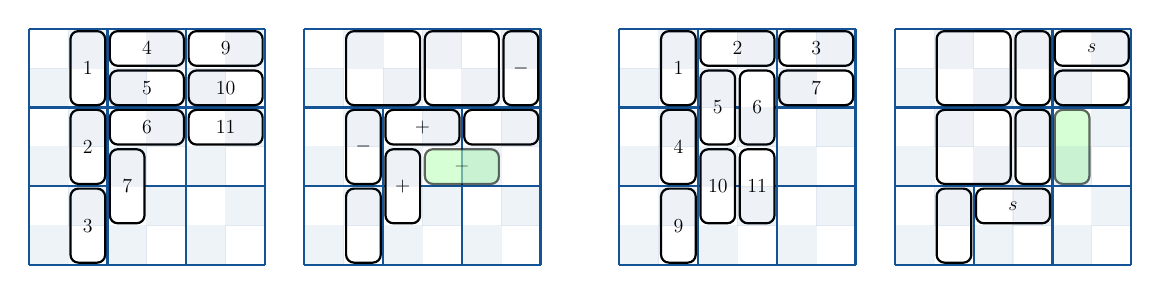
\begin{tikzpicture}[tableau, scale=.5]\gridLines{3}{3}\verticalDomino{1}{2}{1}\verticalDomino{3}{2}{2}\verticalDomino{5}{2}{3}\horizontalDomino{1}{3}{4}\horizontalDomino{2}{3}{5}\horizontalDomino{3}{3}{6}\verticalDomino{4}{3}{7}\horizontalDomino{1}{5}{9}\horizontalDomino{2}{5}{10}\horizontalDomino{3}{5}{11}\fixedSquaresForGrid{3}{3}
        \gridLinesShift{3}{3}{7}
        \verticalDominoShift{3}{2}{-}{7}
        \verticalDominoShift{5}{2}{}{7}
        \horizontalDominoShift{3}{3}{+}{7}
        \emptyBoxShift{1}{2}{7}
        \verticalDominoShift{4}{3}{+}{7}
        \verticalDominoShift{1}{6}{-}{7}
        \horizontalDominoShift{3}{5}{}{7}
        \emptyBoxShift{1}{4}{7}
        \horizontalDominoRSShift{4}{4}{-}{7}
        \fixedSquaresForGridShift{3}{3}{7}
        \gridLinesShift{3}{3}{15}\verticalDominoShift{1}{2}{1}{15}\horizontalDominoShift{1}{3}{2}{15}\horizontalDominoShift{1}{5}{3}{15}\verticalDominoShift{3}{2}{4}{15}\verticalDominoShift{2}{3}{5}{15}\verticalDominoShift{2}{4}{6}{15}\horizontalDominoShift{2}{5}{7}{15}\verticalDominoShift{5}{2}{9}{15}\verticalDominoShift{4}{3}{10}{15}\verticalDominoShift{4}{4}{11}{15}\fixedSquaresForGridShift{3}{3}{15}
        \gridLinesShift{3}{3}{22}
        \verticalDominoShift{1}{4}{}{22}
        \horizontalDominoShift{1}{5}{s}{22}
        \verticalDominoShift{3}{4}{}{22}
        \emptyBoxShift{1}{2}{22}
        \horizontalDominoShift{2}{5}{}{22}
        \verticalDominoShift{5}{2}{}{22}
        \horizontalDominoShift{5}{3}{s}{22}
        \emptyBoxShift{3}{2}{22}
        \verticalDominoRSShift{3}{5}{}{22}
        \fixedSquaresForGridShiftAlt{3}{3}{22}
        \end{tikzpicture}
      \end{figure}
      goes to
      \begin{figure}[H]
        % 1s 2t 3s 5+ 4_6 7s 10- 9_11 8_12
        \centering
        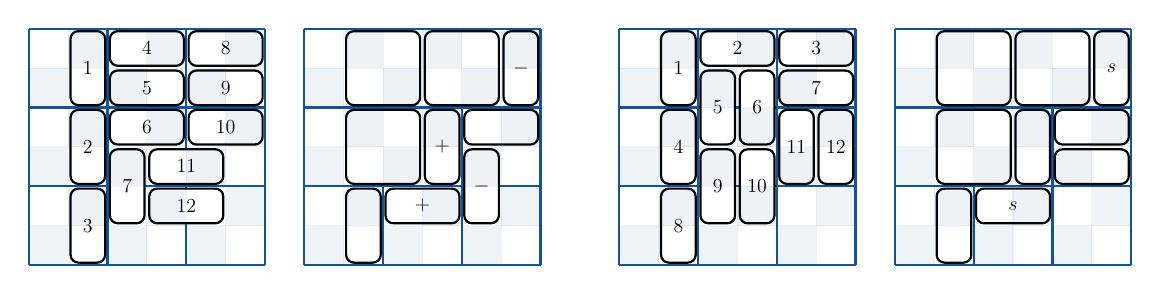
\begin{tikzpicture}[tableau, scale=.5]\gridLines{3}{3}\verticalDomino{1}{2}{1}\verticalDomino{3}{2}{2}\verticalDomino{5}{2}{3}\horizontalDomino{1}{3}{4}\horizontalDomino{2}{3}{5}\horizontalDomino{3}{3}{6}\verticalDomino{4}{3}{7}\horizontalDomino{1}{5}{8}\horizontalDomino{2}{5}{9}\horizontalDomino{3}{5}{10}\horizontalDomino{4}{4}{11}\horizontalDomino{5}{4}{12}\fixedSquaresForGrid{3}{3}\gridLinesShift{3}{3}{7}\verticalDominoShift{5}{2}{}{7}\verticalDominoShift{3}{4}{+}{7}\emptyBoxShift{1}{2}{7}\verticalDominoShift{1}{6}{-}{7}\horizontalDominoShift{3}{5}{}{7}\emptyBoxShift{1}{4}{7}\verticalDominoShift{4}{5}{-}{7}\horizontalDominoShift{5}{3}{+}{7}\emptyBoxShift{3}{2}{7}\fixedSquaresForGridShift{3}{3}{7}\gridLinesShift{3}{3}{15}\verticalDominoShift{1}{2}{1}{15}\horizontalDominoShift{1}{3}{2}{15}\horizontalDominoShift{1}{5}{3}{15}\verticalDominoShift{3}{2}{4}{15}\verticalDominoShift{2}{3}{5}{15}\verticalDominoShift{2}{4}{6}{15}\horizontalDominoShift{2}{5}{7}{15}\verticalDominoShift{5}{2}{8}{15}\verticalDominoShift{4}{3}{9}{15}\verticalDominoShift{4}{4}{10}{15}\verticalDominoShift{3}{5}{11}{15}\verticalDominoShift{3}{6}{12}{15}\fixedSquaresForGridShift{3}{3}{15}\gridLinesShift{3}{3}{22}\verticalDominoShift{1}{6}{s}{22}\verticalDominoShift{3}{4}{}{22}\emptyBoxShift{1}{2}{22}\verticalDominoShift{5}{2}{}{22}\horizontalDominoShift{5}{3}{s}{22}\emptyBoxShift{3}{2}{22}\horizontalDominoShift{4}{5}{}{22}\horizontalDominoShift{3}{5}{}{22}\emptyBoxShift{1}{4}{22}\fixedSquaresForGridShiftAlt{3}{3}{22}\end{tikzpicture}
      \end{figure}

      \item Here the pair domino is blank (with sign $s$ on the dual side) and all the dominoes in its row to its right are also blank.
      We'll give the new domino in the dual tableau a $t$ sign, and then make the new dominoes and their pairs compatible with what is there already.
      Then we'll add an $s$ sign below in the dual tableau.
      Here is an example.
      \begin{figure}[H]
        % 1s 3s 4t 2_-6
        \centering
        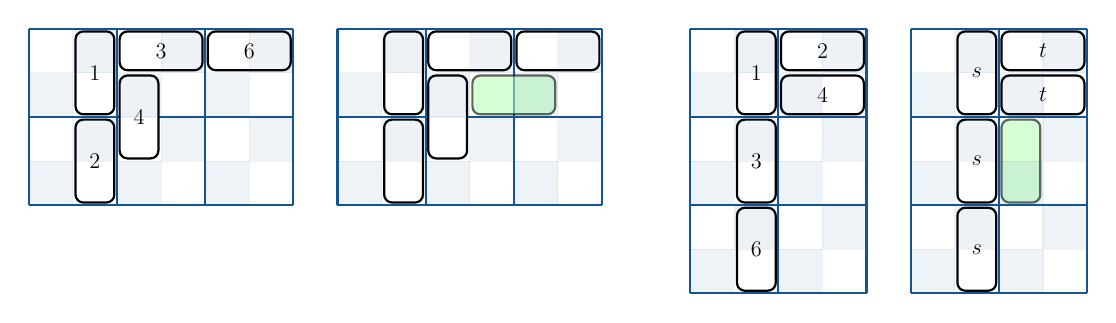
\begin{tikzpicture}[tableau, scale=.56]\gridLines{2}{3}\verticalDomino{1}{2}{1}\verticalDomino{3}{2}{2}\horizontalDomino{1}{3}{3}\verticalDomino{2}{3}{4}\horizontalDomino{1}{5}{6}\fixedSquaresForGrid{2}{3}
        \gridLinesShift{2}{3}{7}
        \horizontalDominoRSShift{2}{4}{}{7}
        \verticalDominoShift{1}{2}{}{7}\horizontalDominoShift{1}{3}{}{7}\verticalDominoShift{3}{2}{}{7}\verticalDominoShift{2}{3}{}{7}\horizontalDominoShift{1}{5}{}{7}\fixedSquaresForGridShift{2}{3}{7}\gridLinesShift{3}{2}{15}\verticalDominoShift{1}{2}{1}{15}\horizontalDominoShift{1}{3}{2}{15}\verticalDominoShift{3}{2}{3}{15}\horizontalDominoShift{2}{3}{4}{15}\verticalDominoShift{5}{2}{6}{15}\fixedSquaresForGridShift{3}{2}{15}\gridLinesShift{3}{2}{20}\verticalDominoShift{1}{2}{s}{20}\verticalDominoShift{3}{2}{s}{20}\horizontalDominoShift{1}{3}{t}{20}\horizontalDominoShift{2}{3}{t}{20}\verticalDominoShift{5}{2}{s}{20}
        \verticalDominoRSShift{3}{3}{}{20}
        \fixedSquaresForGridShiftAlt{3}{2}{20}\end{tikzpicture}
      \end{figure}
      goes to
      \begin{figure}[H]
        % 1s 3s 4t 2_-6 5_7
        \centering
        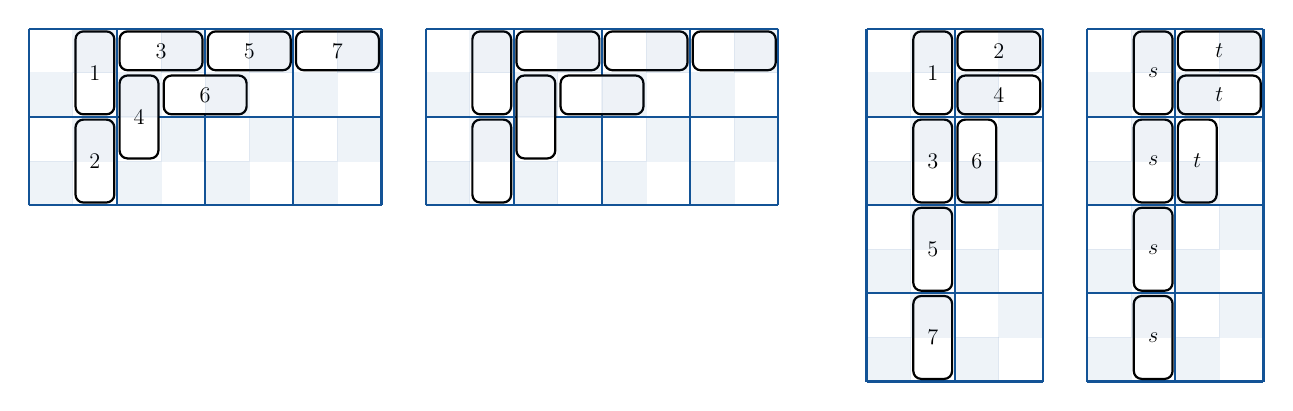
\begin{tikzpicture}[tableau, scale=.56]\gridLines{2}{4}\verticalDomino{1}{2}{1}\verticalDomino{3}{2}{2}\horizontalDomino{1}{3}{3}\verticalDomino{2}{3}{4}\horizontalDomino{1}{5}{5}\horizontalDomino{2}{4}{6}\horizontalDomino{1}{7}{7}\fixedSquaresForGrid{2}{4}\gridLinesShift{2}{4}{9}\verticalDominoShift{1}{2}{}{9}\horizontalDominoShift{1}{3}{}{9}\verticalDominoShift{3}{2}{}{9}\verticalDominoShift{2}{3}{}{9}\horizontalDominoShift{1}{5}{}{9}\horizontalDominoShift{2}{4}{}{9}\horizontalDominoShift{1}{7}{}{9}\fixedSquaresForGridShift{2}{4}{9}\gridLinesShift{4}{2}{19}\verticalDominoShift{1}{2}{1}{19}\horizontalDominoShift{1}{3}{2}{19}\verticalDominoShift{3}{2}{3}{19}\horizontalDominoShift{2}{3}{4}{19}\verticalDominoShift{5}{2}{5}{19}\verticalDominoShift{3}{3}{6}{19}\verticalDominoShift{7}{2}{7}{19}\fixedSquaresForGridShift{4}{2}{19}\gridLinesShift{4}{2}{24}\verticalDominoShift{1}{2}{s}{24}\verticalDominoShift{3}{2}{s}{24}\horizontalDominoShift{1}{3}{t}{24}\horizontalDominoShift{2}{3}{t}{24}\verticalDominoShift{5}{2}{s}{24}\verticalDominoShift{3}{3}{t}{24}\verticalDominoShift{7}{2}{s}{24}\fixedSquaresForGridShiftAlt{4}{2}{24}\end{tikzpicture}
      \end{figure}

      Here is another example.
      \begin{figure}[H]
        % 1s 3+ 4s 2_-6
        \centering
        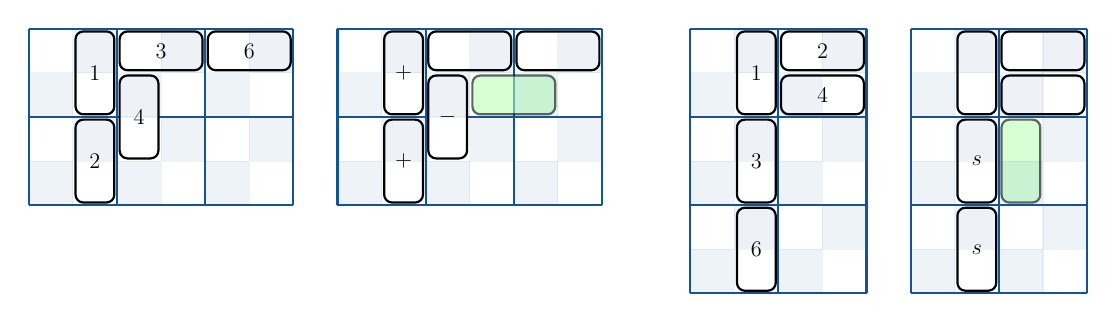
\begin{tikzpicture}[tableau, scale=.56]\gridLines{2}{3}\verticalDomino{1}{2}{1}\verticalDomino{3}{2}{2}\horizontalDomino{1}{3}{3}\verticalDomino{2}{3}{4}\horizontalDomino{1}{5}{6}\fixedSquaresForGrid{2}{3}
        \gridLinesShift{2}{3}{7}
        \horizontalDominoRSShift{2}{4}{}{7}
        \verticalDominoShift{1}{2}{+}{7}\horizontalDominoShift{1}{3}{}{7}\verticalDominoShift{3}{2}{+}{7}\verticalDominoShift{2}{3}{-}{7}\horizontalDominoShift{1}{5}{}{7}\fixedSquaresForGridShift{2}{3}{7}\gridLinesShift{3}{2}{15}\verticalDominoShift{1}{2}{1}{15}\horizontalDominoShift{1}{3}{2}{15}\verticalDominoShift{3}{2}{3}{15}\horizontalDominoShift{2}{3}{4}{15}\verticalDominoShift{5}{2}{6}{15}\fixedSquaresForGridShift{3}{2}{15}\gridLinesShift{3}{2}{20}\verticalDominoShift{1}{2}{}{20}\verticalDominoShift{3}{2}{s}{20}\horizontalDominoShift{1}{3}{}{20}\horizontalDominoShift{2}{3}{}{20}\verticalDominoShift{5}{2}{s}{20}
        \verticalDominoRSShift{3}{3}{}{20}
        \fixedSquaresForGridShiftAlt{3}{2}{20}\end{tikzpicture}
      \end{figure}
      goes to
      \begin{figure}[H]
        % 1s 3+ 4s 2_-6 5_7
        \centering
        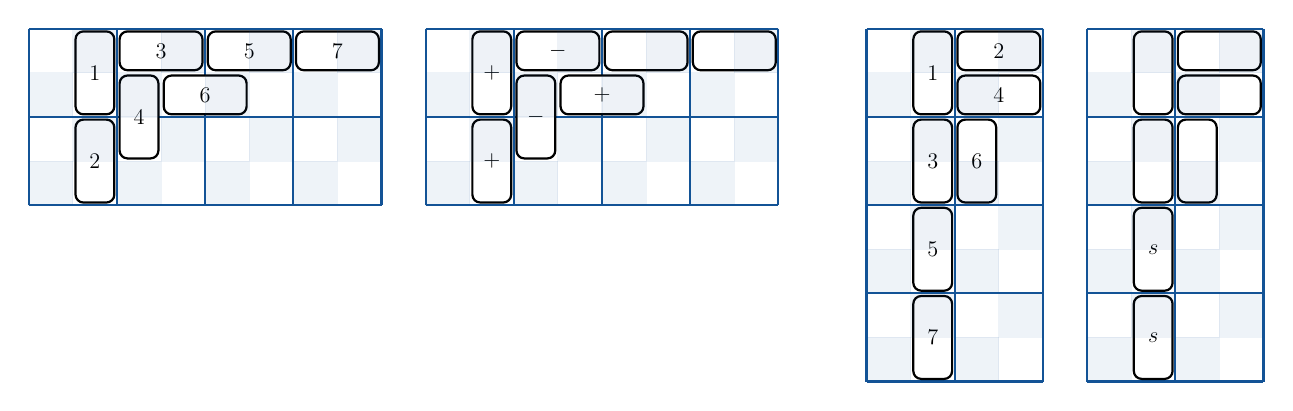
\begin{tikzpicture}[tableau, scale=.56]\gridLines{2}{4}\verticalDomino{1}{2}{1}\verticalDomino{3}{2}{2}\horizontalDomino{1}{3}{3}\verticalDomino{2}{3}{4}\horizontalDomino{1}{5}{5}\horizontalDomino{2}{4}{6}\horizontalDomino{1}{7}{7}\fixedSquaresForGrid{2}{4}\gridLinesShift{2}{4}{9}\verticalDominoShift{1}{2}{+}{9}\horizontalDominoShift{1}{3}{-}{9}\verticalDominoShift{3}{2}{+}{9}\verticalDominoShift{2}{3}{-}{9}\horizontalDominoShift{1}{5}{}{9}\horizontalDominoShift{2}{4}{+}{9}\horizontalDominoShift{1}{7}{}{9}\fixedSquaresForGridShift{2}{4}{9}\gridLinesShift{4}{2}{19}\verticalDominoShift{1}{2}{1}{19}\horizontalDominoShift{1}{3}{2}{19}\verticalDominoShift{3}{2}{3}{19}\horizontalDominoShift{2}{3}{4}{19}\verticalDominoShift{5}{2}{5}{19}\verticalDominoShift{3}{3}{6}{19}\verticalDominoShift{7}{2}{7}{19}\fixedSquaresForGridShift{4}{2}{19}\gridLinesShift{4}{2}{24}\verticalDominoShift{1}{2}{}{24}\verticalDominoShift{3}{2}{}{24}\horizontalDominoShift{1}{3}{}{24}\horizontalDominoShift{2}{3}{}{24}\verticalDominoShift{5}{2}{s}{24}\verticalDominoShift{3}{3}{}{24}\verticalDominoShift{7}{2}{s}{24}\fixedSquaresForGridShiftAlt{4}{2}{24}\end{tikzpicture}
      \end{figure}
    \end{itemize}
  \end{itemize}
\end{document}
